\chapter{Two-Phase Locking is Serializable}

The idea of enabling client reasoning around \tpl\ using the style proposed by mCAP is only feasible once we are able to prove the logic's soundness with respect to the operational semantics for two-phase locking. This objective will guide us through the entirety of this section that gradually defines and proves all of the necessary components. We take a multi-step approach in proving soundness, by first showing the equivalence between the \tpl\ semantics and the \textsc{Atom} semantics, where transactions are ran in one single step by reducing their body to termination. This result is achieved using a strategy that requires the serializability of two-phase locking, together with a set of properties that will be analysed in detail. Next, it is also shown that mCAP's original operational semantics, directly inherited from the Views framework \cite{views}, are able to replicate any execution that can happen through the \textsc{Atom} ones. We can now see how the entire strategy fits together and will be utilized to finally complete the soundness proof.

\subsection{Serializability}

The operational semantics for \tpl\ defined in Section \ref{sec:2plSemantics} claim that, given the adherence to the two phase protocol, they guarantee the serializability of the histories of operations that arise from program executions. This section is dedicated to proving such statement by analyzing traces produced by programs. We begin with some preliminary definitions followed by auxiliary lemmata and finally a proof of serializability following the guidelines in \cite{ccontrol}.

\subsubsection{Traces}

Since serializability is a property of program histories our proof will use them and we therefore here introduce and formalize the concept of a trace.

\begin{defn}
	(Trace).
	A \emph{trace} is an ordered sequence of operations that are generated by the reduction of a generic program under the \tpl\ semantics. It comes from the set $[\mathsf{Act} \times \mathds{N}]$ which is ranged over by $\tau, \tau_1, \ldots, \tau_n$. Every element of a trace is a tuple with an action label and an ordinal number to represent the numerical index of the operation.
\end{defn}

We refer to elements of a trace as operations, often using $op, x, y$ to range over them. We only study the particular kind of traces that arises from a program which succesfully terminates and reduces to $\pskip$. Such traces can be retrieved from program executions using the $\mathsf{trace}$ function, that given a storage, transactions stack and program, returns one of the possible traces that are produced by the operational semantics starting with the input state.
\begin{align*}
	\pred{trace}{h, \Phi, S, \mathds{P}} &\triangleq \pred{trace'}{h, \Phi, S, \mathds{P}, 0} \\
	\pred{trace'}{h, \emptyset, S, \pskip, n} &\triangleq [] \\
	\pred{trace'}{h, \Phi, S, \mathds{P}, n} &\triangleq (\alpha, n) : \pred{trace'}{h', \Phi', S', \mathds{P}', n+ 1}
	\\
	\text{where }& (h, \Phi, S, \mathds{P}) \xrightarrow{\alpha} (h', \Phi', S', \mathds{P}') \rightarrow^* (h'', \emptyset, S'', \pskip)
\end{align*}

To better illustrate concrete traces we provide an example program with its corresponding formally generated trace. Consider the program and trace in Figure. The first transaction assigns $5$ value to variable $\pvar{x}$ and later mutates the same cell to write value $2$. The other one checks whether cell indexed with $5$ has a value of $2$ and if so, it updates it back to $0$. In the execution preliminaries, the two user transactions get converted into system one and are assigned with identifiers, $4$ and $1$ respectively. Later, transaction $4$ acquires the lock on $5$ in exclusive mode, meaning it will complete the reduction of its commands before $1$ starts with its own ones. since it needs the same lock in shared mode first, then in the exclusive one to complete the update.

\[
	\begin{array}{l r}
		\begin{array}{l || l}
			\begin{array}{l}
				\mathtt{begin} \\
					\quad \passign{\pvar{x}}{5} ; \\
					\quad \pmutate{\pvar{x}}{2} \\
				\mathtt{end}
			\end{array}
				&
			\begin{array}{l}
				\mathtt{begin} \\
					\quad \pderef{\pvar{y}}{5} ; \\
					\quad \pifs{\pvar{y} = 2} \\
					\quad \quad \pmutate{5}{0} \\
					\quad \pifm \\
					\quad \quad \pskip \\
				\mathtt{end}
			\end{array}
		\end{array}
		&
		\begin{array}{r l}
			\tau =
			&
			\left[
			\begin{aligned}
				&(\actid{1}, 0), (\actid{4}, 1), (\actid{4}, 2), (\actlock{4}{5}{\textsc{x}}, 3), \\
				&(\actid{4}, 4), (\actwrite{4}{5}{2}, 5), (\actunlock{4}{5}, 6), \\
				&(\actlock{1}{5}{\textsc{s}}, 7), (\actid{4}, 8), (\actread{1}{5}{2}, 9), \\
				&(\actid{4}, 10), (\actid{4}, 11), (\actlock{1}{5}{\textsc{x}}, 12), \\
				&(\actwrite{1}{5}{0}, 13),  (\actunlock{1}{5}, 14), \\
				&(\actid{4}, 15), (\actprog, 16)
			\end{aligned}
			\right]
		\end{array}
	\end{array}
\]

Going back to formal definitions, we say that an operation $op \in \mathsf{Act} \times \mathds{N}$ belongs to a trace $\tau$, written $op \in \tau$ if and only if $op \in \tau = \top$ where the $\in$ function is defined as follows:
\begin{align*}
	(\alpha, n) \in [] &\triangleq \bot \\
	(\alpha, n) \in (\alpha, n):\tau &\triangleq \top \\
	(\alpha, n) \in (\alpha', n'):\tau &\triangleq (\alpha, n) \in \tau
\end{align*}

It is often useful to express the order of operations as part of a trace. For this reason, we introduce the precedence of operations which asserts that two operations belong to the trace and their respective indexes are correctly ordered.
\begin{defn}
	(Operation precedence).
	The \emph{operation precedence} as part of a trace $\tau$, written $\tau \vDash x < y$, is defined in the following way:
	\[
		\tau \vDash (\alpha, n) < (\alpha', n') \overset{\text{def}}{\iff}
(\alpha, n) \in \tau \land (\alpha', n') \in \tau \land n < n'
	\]
\end{defn}

For conciseness, we overload the definition of $<$ to cope with the ordering of a concrete operation and a generic action (i.e. the first component of an operation) and of two generic actions without an associated index.
\begin{align*}
	\tau \vDash op < \alpha \overset{\text{def}}{\iff}&
	\exists n \ldotp \tau \vDash op < (\alpha, n)
		\\
	\tau \vDash \alpha < op \overset{\text{def}}{\iff}&
	\exists n \ldotp \tau \vDash (\alpha, n) < op
		\\
	\tau \vDash \alpha < \alpha' \overset{\text{def}}{\iff}&
	\exists n, n' \ldotp \tau \vDash (\alpha, n) < (\alpha', n')
\end{align*}

This allows to assert on the existence of some particular action appearing before or after another one as part of a trace which will prove very useful in proofs. Two different actions which are part of the same trace are in conflict if they are performed by different transactions and one of them is a write or alloc while the other one is a read, write or alloc on the same key. These are treated specially since the order in which they appear might affect the end result of the program execution.

\begin{defn}
	\label{defn:conflict}
	(Conflicting actions).
	Actions $\alpha$ and $\alpha'$ are \emph{conflicting} if and only if they both belong to the same trace $\tau$ and $\pred{conflict}{\alpha, \alpha'} = \top$, where the $\mathsf{conflict}$ function is defined as:
	\begin{align*}
		\pred{conflict}{\actwrite{i}{k}{v}, \actwrite{j}{k}{v'}} &\triangleq i \neq j
			\\
		\pred{conflict}{\actwrite{i}{k}{v}, \actread{j}{k}{v'}} &\triangleq i \neq j
			\\
		\pred{conflict}{\actread{i}{k}{v}, \actwrite{j}{k}{v'}} &\triangleq i \neq j
			\\
		\pred{conflict}{\actalloc{i}{n}{l}, \actread{j}{k}{v'}} &\triangleq i \neq j \land l \leq k < l + n
			\\
		\pred{conflict}{\actalloc{i}{n}{l}, \actwrite{j}{k}{v'}} &\triangleq i \neq j \land l \leq k < l + n
			\\
		\pred{conflict}{\alpha, \alpha'} &\triangleq \bot
	\end{align*}
\end{defn}
We overload Definition \ref{defn:conflict} to also cope with trace operations, by simply unwrapping them and extracting the corresponding action part of the tuple.
\[
	\pred{conflict}{(\alpha, n), (\alpha', n')} \triangleq \pred{conflict}{\alpha, \alpha'}
\]

Finally, in order to aid the clarity of property definitions regarding traces, we define two predicates describing particular operations. The first one, $op(\iota)$, refers to any action performed by transaction $\mathds{T}_\iota$.
\begin{align*}
	op(\iota) \triangleq (\alpha, n) \text{ s.t. } \alpha \in \{ &\actid{\iota}, \actwrite{\iota}{k}{v}, \actlock{\iota}{k}{\kappa}, \actunlock{\iota}{k}, \actread{\iota}{k}{v},
	\\
	&\actalloc{\iota}{m}{l}\ |\ k, l \in \mathsf{Key}, v \in \mathsf{Val}, n \in \mathds{N}, \kappa \in \mathsf{Lock}, m \in \mathds{N} \} \land n \in \mathds{N} \}
\end{align*}
Similarly, the $op(\iota, k)$ predicate describes any operation done by the transaction identified with $\iota$, which accesses item $k$, i.e. either reading, writing or allocating it.
\begin{align*}
	op(\iota, k) \triangleq (\alpha, n) \text{ s.t. } \alpha \in\ &\{ \actread{\iota}{k}{v}, \actwrite{\iota}{k}{v}\ |\ v \in \mathsf{Val} \}\
	\cup \\
	&\{\actalloc{\iota}{m}{l}\ |\ m \in \mathds{N}, l \in \mathsf{Key}, l \leq k < l + m \} \land n \in \mathds{N}
\end{align*}

The two following definitions empower us to formally define the serializability of traces. We start by describing what it means for a trace $\tau$ to be serial: intuitively, $\tau$ is the result of running a program where transactions are executed in a sequential fashion, with no interleaving of operations. Next, we define the concept of equivalence between traces. This is expressed by imposing the equality on their operations and transactions, but not strictly on the order in which they appear. In fact, only conflicting operations are required to be ordered in the same way.

\begin{defn}
	(Trace equivalence).
	Two traces $\tau, \tau' \in [\mathsf{Act} \times \mathds{N}]$ are defined to be \emph{equivalent}, written $\tau \equiv \tau'$, if and only if they contain the same transactions and operations and if they order conflicting operations in the same way.
	\begin{gather*}
		\tau \equiv \tau' \iff \\
		(\forall \iota, x \ldotp x = op(\iota) \lor x = \actprog \implies (x \in \tau \iff x \in \tau'))\ \land \\
		(\forall x, x', i, j, k \ldotp x = op(i, k) \land x' = op(j, k) \land \pred{conflict}{x, x'}
		\implies (\tau \vDash x < x' \iff \tau' \vDash x < x'))
	\end{gather*}
\end{defn}

\begin{defn}
	(Serial trace).
	A trace $\tau$ is defined as \emph{serial} if and only if for any two transactions, $i$ and $j$, inside of it either all of $i$'s operations appear before $j$'s ones or all of $j$'s operations appear before $i$'s ones.
	\begin{gather*}
		\pred{serial}{\tau} \iff \\
		\forall i, j \ldotp i \neq j \land op(i) \in \tau \land op(j) \in \tau \implies \\
		(\forall x, x' \ldotp x = op(i) \in \tau \land x' = op(j) \in \tau \implies \tau \vDash x < x') \\
		\lor \\
		(\forall x, x' \ldotp x = op(i) \in \tau \land x' = op(j) \in \tau \implies \tau \vDash x' < x)
	\end{gather*}
\end{defn}

\begin{defn}
	(Serializable).
	A trace $\tau$ is \emph{serializable} if and only if it is equivalent to some serial trace $\tau'$.
	\[
		\pred{serializable}{\tau} \iff \exists \tau' \ldotp \pred{serial}{\tau'} \land \tau \equiv \tau'
	\]
\end{defn}

\begin{center}
	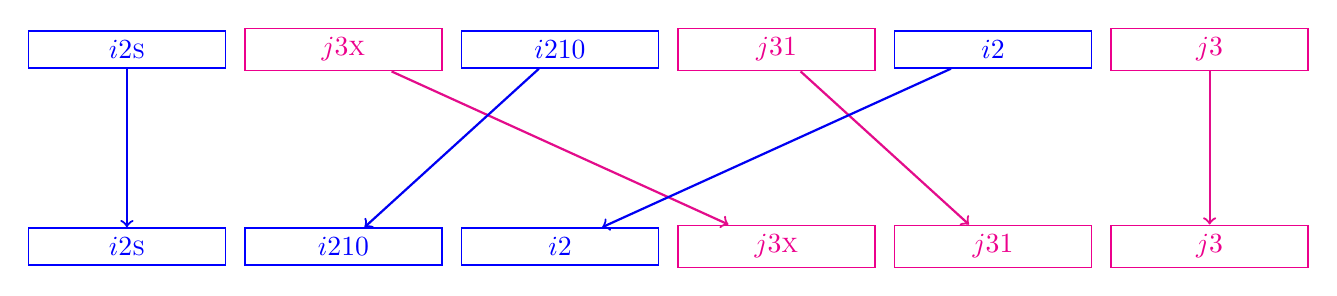
\begin{tikzpicture}[->, semithick]
		\tikzset{
		    tleft/.style= {rectangle, draw=blue, color=blue, minimum width=2.5cm},
		    tright/.style= {rectangle, draw=magenta, color=magenta, minimum width=2.5cm},
		    pleft/.style= {above, black!5!blue, thick},
		    pright/.style= {above, black!5!magenta, thick},
		}
		
		\node[tleft] (s1) at (0, 0) {$\actlock{i}{2}{\textsc{s}}$};
		\node[tright] (s2) at (2.75, 0) {$\actlock{j}{3}{\textsc{x}}$};
		\node[tleft] (s3) at (5.5, 0) {$\actread{i}{2}{10}$};
		\node[tright] (s4) at (8.25, 0) {$\actwrite{j}{3}{1}$};
		\node[tleft] (s5) at (11, 0) {$\actunlock{i}{2}$};
		\node[tright] (s6) at (13.75, 0) {$\actunlock{j}{3}$};
		
		\node[tleft] (s7) at (0,-2.5) {$\actlock{i}{2}{\textsc{s}}$};
		\node[tleft] (s8) at (2.75,-2.5) {$\actread{i}{2}{10}$};
		\node[tleft] (s9) at (5.5,-2.5) {$\actunlock{i}{2}$};
		\node[tright] (s10) at (8.25,-2.5) {$\actlock{j}{3}{\textsc{x}}$};
		\node[tright] (s11) at (11,-2.5) {$\actwrite{j}{3}{1}$};
		\node[tright] (s12) at (13.75,-2.5) {$\actunlock{j}{3}$};
		
		\draw
		(s1) edge[pleft] (s7)
		(s2) edge[pright] (s10)
		(s3) edge[pleft] (s8)
		(s4) edge[pright] (s11)
		(s5) edge[pleft] (s9)
		(s6) edge[pright] (s12);
	\end{tikzpicture}
	\captionof{figure}{A serializable trace at the top with the corresponding equivalent and serial trace.}
\end{center}

\subsubsection{Graphs}

The proof of serializability will be carried over a particular representation of traces that we introduce in this section. We utilize serialization graphs in order to describe relationships between transactions participating in a program execution.

\begin{defn}
	(Serialization graph).
	The \emph{serialization graph} of a given trace $\tau$ is a directed graph whose nodes are the identifiers of all the transactions that perform an action as part of $\tau$ and whose edges are between transactions that have ordered conflicting operations according to $\tau$.
	\begin{align*}
		\pred{SG}{\tau} &\triangleq (N, E) \\
		\text{where } N &\triangleq \{ \iota\ |\ op(\iota) \in \tau \} \\
		E &\triangleq
			\begin{aligned}
				\{
					(i, j)\ |&\ x = op(i, k) \land x' = op(j, k) \\
					&\land \pred{conflict}{x, x'} \land \tau \vDash x < x' 
				\}	
			\end{aligned}
	\end{align*}
\end{defn}

Edge connections and paths within a graph $G = (N, E)$ are described by introducing an arrow notation. We write $i \rightarrow j \in G$ to indicate that there is an edge from node $i$ to node $j$ in $E$. In the following list of statements, we make an abuse of notation to allow more expressive formulas and add a transitive closure arrow ($\rightarrow^*$) that is able to describe a path in the graph.
\[
	\begin{array}{l l}
		i \rightarrow j \in E \triangleq (i, j) \in E
			&
		i \rightarrow j \in G \triangleq i \rightarrow j \in G \downarrow_2
			\\
		i \rightarrow^1 j \in E \triangleq i \rightarrow j \in E
			&
		i \rightarrow^n j \in E \triangleq \exists t \ldotp i \rightarrow t \in E \land t \rightarrow^{n-1} \in E
			\\
		i \rightarrow^* j \in E \triangleq \exists n \ldotp i \rightarrow^n j \in E
			\ \ \ \ &
		i \rightarrow^* j \in G \triangleq i \rightarrow^* j \in G \downarrow_2
	\end{array}		
\]

Our goal is now to prove that all traces whose serialization graph contains no cyclic paths are serializable. We do this by first formally introducing the acyclic property of graphs and later the concept of a topological order of a graph.

\begin{defn}
	(Acyclic graph).
	A graph $G = (N, E)$ is \emph{acyclic} if and only if there is no path in $G$ that connects a node in $N$ to itself.
	\[
		\pred{acyclic}{G} \iff \forall a \ldotp a \in G \downarrow_1 \implies \lnot a \rightarrow^* a \in G
	\]
\end{defn}

\begin{defn}
	(Topological sort).
	A \emph{topological sort} of a graph $G = (N, E)$ is an ordered sequence of all nodes in $N$ such that if node $a$ appears before node $b$ in the sequence, then there is no path from $b$ to $a$ in $G$.
	\begin{gather*}
		t = \pred{topo}{(N, E)} \iff \\
		(\forall n \ldotp n \in t \iff n \in N) \land (\forall a, b \ldotp t \vDash a < b \implies \lnot b \rightarrow^* a \not\in E)
	\end{gather*}
\end{defn}

The following theorem establishes a key property we later need in order to prove serializability of the operational semantics introduced in Section \ref{sec:2plSemantics}. The process will in fact start by building the serialization graph of an arbitrary trace arising from \tpl\ semantics, showing that under any circumstance it is acyclic and from Theorem \ref{thm:acySer} we obtain the result needed.
\begin{thm}
	\label{thm:acySer}
	(Acyclic means serializable).
	Every trace that has a serialization graph with no cycles is serializable.
	\[
		\forall \tau \ldotp \pred{acyclic}{\pred{SG}{\tau}} \implies \pred{serializable}{\tau}
	\]
	
	\begin{proof}
	Let's assume that $\tau \in [\mathsf{Act} \times \mathds{N}]$ is a trace which includes operations coming from transactions identified with $N = \{ \iota_1, \ldots, \iota_m \}$ for a finite $m$. It follows that $N$ is also the set of nodes of $\pred{SG}{\tau}$. By our original assumption we know that $\pred{SG}{\tau}$ is acyclic. For this reason we can always find a topological sort $t = \pred{topo}{\pred{SG}{\tau}} = [t_{\iota_1}, \ldots, t_{\iota_m}]$. Let $\tau'$ be the serial trace that includes transactions (in the presented order) identified with $t_{\iota_1}, \ldots, t_{\iota_m}$ and has all of the same operations as $\tau$. Let $x = op(i, k)$ and $x' = op(j, k)$ such that $\pred{conflict}{x, x'}$ holds and $\tau \vDash x < x'$. By definition of serialization graph, $i \rightarrow j \in \pred{SG}{\tau}$. Therefore, in any topological sort of $\pred{SG}{\tau}$, $i$ must appear before $j$. As a consequence, all of $i$'s operations appear before $j$'s ones in $\tau'$ and in particular $\tau' \vDash x < x'$. By construction, $\tau'$ is serial and it contains all of $\tau$'s operations and we showed that any two conflicting operations are ordered in the same way. We can conclude that $\tau \equiv \tau'$ which implies that $\tau$ is serializable.
	\end{proof}
\end{thm}

\subsubsection{Proof}

\begin{lem}
	All read, write or alloc operations are followed by an unlock action on the same key done by the same transaction.
	\[
		\forall \tau, \iota, k, \kappa, x \ldotp
		x = op(\iota, k) \land x \in \tau \implies \left( \tau \vDash x < \actunlock{\iota}{k} \right)
	\]
\end{lem}

\begin{lem}
	All reads are preceded by the appropriate shared lock acquisition.
	\begin{gather*}
		\forall \tau, \iota, k, v, \kappa, x, n \ldotp \\
		x = (\actread{\iota}{k}{v}, n) \land x \in \tau \implies \left( \tau \vDash \actlock{\iota}{k}{\kappa} < x \land \kappa \geq \textsc{s} \right)
	\end{gather*}
\end{lem}

\begin{lem}
	All writes to a cell are preceded by the appropriate exclusive lock acquisition.
	\begin{gather*}
		\forall \tau, x, i, k, v, n \ldotp
		x = (\actwrite{i}{k}{v}, n) \land x \in \tau \implies
		\tau \vDash \actlock{i}{k}{\textsc{x}} < x
	\end{gather*}
\end{lem}

\begin{lem}
	A read or write operation accessing a cell allocated as part of the trace, must appear after the corresponding alloc action.
	\begin{gather*}
		\forall \tau, i, j, x, x', n, n', l, m, k, v, \kappa \ldotp \\
		x = (\actalloc{i}{m}{l}, n) \land x' \in \{ (\actread{j}{k}{v}, n'), (\actwrite{j}{k}{v}, n') \} \land l \leq k < l + m
		\\
		\land x \in \tau \land x' \in \tau
		\implies
		\left( \tau \vDash x < x'  \land \tau \vDash \actunlock{i}{k} < \actlock{j}{k}{\kappa} \right)
	\end{gather*}
\end{lem}

\begin{lem}
	No lock is acquired by a transaction after one gets released by the same transaction.
	\begin{gather*}
		\forall \tau, \iota, k, k', n, n', x, x', \kappa \ldotp \\
		\left( x = (\actlock{\iota}{k}{\kappa}, n) \land x' = (\actunlock{\iota}{k'}, n') \land x \in \tau \land x' 	\in \tau \right) \\
		\implies \left( \tau \vDash x < x' \right)
	\end{gather*}
\end{lem}

\begin{lem}
	If two transactions run conflicting operations on the same item, either one releases its lock before the other acquires it or vice versa.
	\begin{gather*}
		\forall \tau, i, j, k, \kappa, \kappa', x, x' \ldotp \\
		x = op(i, k) \in \tau \land x' = op(j, k) \in \tau \land \pred{conflict}{x, x'} \\
		\implies \left( \tau \vDash \actunlock{i}{k} < \actlock{j}{k}{\kappa} \right) \lor \left( \tau \vDash \actunlock{j}{k} < \actlock{i}{k}{\kappa'} \right)
	\end{gather*}
\end{lem}

\lem \label{lem:sg1}
\begin{gather*}
\forall \tau, i, j \ldotp i \rightarrow j \in \pred{SG}{\tau} \implies \\
\exists k, \kappa, x, x' \ldotp x = op(i, k) \in \tau \land x' = op(j, k) \in \tau \\
\land\ \pred{conflict}{x, x'} \land \tau \vDash \actunlock{i}{k} < \actlock{j}{k}{\kappa}
\end{gather*}
\begin{proof}
Let's pick an arbitrary trace $\tau \in [(\mathsf{Act}, \mathds{N})]$, such that $\tau = \pred{trace}{h, \emptyset, \emptyset, \mathds{P}}$ for some $h \in \mathsf{Storage}$, $\mathds{P} \in \mathsf{Prog}$ and transaction identifiers $i, j \in \mathsf{Tid}$. Now we assume that $i \rightarrow j \in \pred{SG}{\tau}$. By definition of a serialization graph built through $\mathsf{SG}$ we directly obtain that there must be two operations $x = op(i, k)$ and $x' = op(j, k)$ in $\tau$ which are conflicting, so $\pred{conflict}{x, x'}$ holds and $\tau \vDash x < x'$ (\textsc{i}).

In the case where $x = (\actalloc{i}{n}{l}, n')$ for some $n, n' \in \mathds{N}$, then we obtain the needed result from Lemma \ref{lem:allocBefore}.

Otherwise $x$ and $x'$ are conflicting read/write operations. By Lemma \ref{lem:read}, Lemma \ref{lem:write} and Lemma \ref{lem:unlock} we obtain the following, for $x_i^l = (\actlock{i}{k}{\kappa}, n_1), x_i^u = (\actunlock{i}{k}, n_2), x_j^l = (\actlock{j}{k}{\kappa'}, n_3), x_j^u = (\actunlock{j}{k}, n_4)$ and $n_1, n_2, n_3, n_4 \in \mathds{N}, \kappa, \kappa' \in \mathsf{Lock}$.
\begin{enumerate}
	\item \label{sg1.1} $\tau \vDash x_i^l < x < x_j^u$
	\item \label{sg1.2} $\tau \vDash x_j^l < x' < x_j^u$
\end{enumerate}
By Lemma \ref{lem:conflict} we know that either $\tau \vDash x_i^u < x_j^l$ or $\tau \vDash x_j^u < x_i^l$ holds. In the case where $\tau \vDash x_j^u < x_i^l$ holds, by points \ref{sg1.1} and \ref{sg1.2} we would get that $\tau \vDash x' < x$ which contradicts (\textsc{i}). Therefore it must be the case that $\tau \vDash x_i^u < x_j^l$ holds.
\end{proof}

\lem \label{lem:sg2}
\begin{gather*}
\forall \tau, i, j, n > 0 \ldotp i \rightarrow^n j \in \pred{SG}{\tau} \implies \\
\exists k, k', \kappa \ldotp op(i, k) \in \tau \land op(j, k') \in \tau \land \tau \vDash \actunlock{i}{k} < \actlock{j}{k}{\kappa}
\end{gather*}

{\parindent0pt
\begin{proof}
Let's pick an arbitrary trace $\tau \in [(\mathsf{Act}, \mathds{N})]$, such that $\tau = \pred{trace}{h, \emptyset, \emptyset, \mathds{P}}$ for some $h \in \mathsf{Storage}$, $\mathds{P} \in \mathsf{Prog}$, $n \in \mathds{Z}$ such that $n > 0$ and transaction identifiers $i, j \in \mathsf{Tid}$. We will prove the lemma by induction on $n$. \\

\textit{Base case}: $n = 1$

We assume that $i \rightarrow^1 j \in \pred{SG}{\tau}$ which, by definition, is equivalent to $i \rightarrow j \in \pred{SG}{\tau}$. By Lemma \ref{lem:sg1} we get that $\exists k, \kappa \ldotp \alpha_i(k) \in \tau \land \alpha_j(k) \in \tau \land \tau \vDash \actunlock{i}{k} < \actlock{j}{k}{\kappa}$ that concludes the proof for this case. \\

\textit{Inductive case}: $n > 1$

\textit{Inductive hypothesis}: Assume the property holds for $n$.

We now want to prove the same property for $n + 1$ so we assume that $i \rightarrow^{n+1} j \in \pred{SG}{\tau}$. By definition, we know that for $n$ and some $t \in \mathsf{Tid}$, $i \rightarrow^n t \in \pred{SG}{\tau}$ and $t \rightarrow j \in \pred{SG}{\tau}$ holds. By inductive hypothesis on $n$ we obtain that, for keys $k_1, k_2 \in \mathsf{Key}$ and lock mode $\kappa_t \in \mathsf{Lock}$, there are two operations $op(i, k_1)$ and $op(t, k_2)$ which are part of $\tau$ and that $\tau \vDash \actunlock{i}{k_1} < \actlock{t}{k_2}{\kappa_t}$ holds. By the fact that $t \rightarrow j \in \pred{SG}{\tau}$ holds and Lemma \ref{lem:sg1} we know that, for a storage key $k \in \mathsf{Key}$ and lock mode $\kappa \in \mathsf{Lock}$, there are two conflicting actions $op(t, k)$ and $op(j, k)$ inside $\tau$ such that $\tau \vDash \actunlock{t}{k} < \actlock{j}{k}{\kappa}$. By Lemma \ref{lem:2phase} we obtain that $\tau \vDash \actlock{t}{k_2}{\kappa_t} < \actunlock{t}{k}$ holds. As a consequence, it follows that $\tau \vDash \actunlock{i}{k_1} < \actlock{j}{k}{\kappa}$.
\end{proof}
}

\thm \label{thm:sgAcyclic}
\[
\forall \tau, i \ldotp i \in \pred{SG}{\tau} \downarrow_1 \implies \lnot i \rightarrow^* i \in \pred{SG}{\tau}
\]

\begin{proof}
Let's pick an arbitrary trace $\tau \in [(\mathsf{Act}, \mathds{N})]$, such that $\tau = \pred{trace}{h, \emptyset, \emptyset, \mathds{P}}$ for some $h \in \mathsf{Storage}$, $\mathds{P} \in \mathsf{Prog}$ and transaction identifier $i \in \mathsf{Tid}$. We assume that $i$ is part of the transaction identifiers in the serialization graph, i.e. $i \in \pred{SG}{\tau} \downarrow_1$. Let's also assume that the graph contains a cycle on $i$, which means that $\exists n \ldotp i \rightarrow^n i \in \pred{SG}{\tau}$. By Lemma \ref{lem:sg2} we obtain that for some keys $k, k' \in \mathsf{Key}$ and lock mode $\kappa \in \mathsf{Lock}$, $\tau \vDash \actunlock{i}{k} < \actlock{i}{k'}{\kappa}$ which contradicts Lemma \ref{lem:2phase}. Therefore, by contradiction we get that $\lnot i \rightarrow^* i \in \pred{SG}{\tau}$.
\end{proof}

\subsection{Semantics Equivalence}

\label{sec:semEquiv}

Serializability gives us an important consistency property on the \tpl\ operational semantics that we defined. In abstract terms, it allows us to think about program executions in some sequential order, without having to consider all possible interleavings that may arise. At this point, we want to show an even stronger result which is the semantics equivalence between the semantics defined in Section \ref{sec:2plSemantics} and some \textit{atomic} operational semantics, defined in Section \ref{sec:atomicSem}, that reduce transactions in one go, as if the system stops when they begin execution and starts again when they are done. In database terms, this is referred to as \textit{strict serializability}, where, on top of order between parallel transactions, the internal program order is also preserved. The equivalence not only allows us to forget about the peculiar locking details of \tpl\ and thus only to focus on \textit{atomic} reductions, but also provides us with soundness with respect to the mCAP program logic defined in Section \ref{sec:mcapModel}. This empowers us to build mCAP proofs of programs running under the \tpl\ semantics.

The final outcome of this section will be a proof of the following statement, which says that any program that terminates, i.e. reduces to $\pskip$, under the \tpl\ operational semantics will have the same overall effect on the global storage as the same terminating program running under the \textsc{Atom} semantics and starting with the same state.
\[
	\forall h, h', S, S', \mathds{P} \ldotp
	(h, \emptyset, S, \mathds{P}) \rightarrow^* (h', \emptyset, S', \pskip) \implies 
	(h, \mathds{P}) \tred^* (h', \pskip)
\]

In order for the semantics equivalence claim to be complete, the inverse implication also needs to be established. This states that the final storage of any terminating program reduction in \textsc{Atom}, will be reachable by reducing the same program starting from the same initial state in \textsc{2pl}, where the transactions' state components are existentially quantified.
\[
	\forall h, h' \ldotp
	(h, \mathds{P}) \tred^* (h', \pskip)
	\implies
	\exists S, S' \ldotp
	(h, \emptyset, S, \mathds{P}) \rightarrow^* (h', \emptyset, S', \pskip)
\]
We do not formally prove this result given that it is trivial to understand that the \textsc{Atom} semantics can be replicated by the \tpl\ ones, simply by always chosing to reduce the same transaction until it reaches $\pskip$, without allowing concurrent interleaving. Given that we start with an empty lock manager component $\emptyset$, run transactions one after the other and each of those needs to remove its footprint from locks before terminating, no transaction will get \textit{stuck} as part of the overall reduction.

\subsubsection{Atomic semantics}

\label{sec:atomicSem}

The atomic operational semantics shown here are behaviourally equivalent to the ones presented in Section \ref{sec:mcapOpSem}. They are converted to a transition relation for clarity and in order to ease the general proof, since the \tpl\ semantics are also expressed with a comparable structure.

The rules that follow determine a relation between storages under the effect of a program. At the level of programs, they are very similar to the \tpl\ ones, a part from the absence of a lock manager or a transactions stack. These two structures are not needed here, since there is no interleaving which happens as a result of running transactions concurrently. For this reason, there is no need to globally track information about a transaction's internal execution. Note how such behaviour is obtained through the \textsc{AtExec} rule, which reduces a transaction's body at once, by running a multi-step reduction on command $\mathds{C}$ until it hits $\pskip$. Parallelism is again obtained by nondeterministically reducing one of the two programs that are composed together.

\[
(-, -) \rightarrow (-, -) : (\mathsf{Storage} \times \mathsf{Prog})^2
\]
\[\footnotesize\def\arraystretch{3.5}
	\begin{array}{c c}
		\infer[\textsc{AtTrans}]
		{
			(h, \mathds{T}) \tred (h', \pskip)
		}
		{
			(h, \mathds{T}) \tred (h', \ptdef{\pskip})
		}
		&
		\infer[\textsc{AtPSkip}]
		{
			(h, \pskip ; \mathds{P}) \tred (h, \mathds{P})
		}
		{}
		\\
		\infer[\textsc{AtPSeq}]
		{
			(h, \mathds{P}_1 ; \mathds{P}_2) \tred (h', \mathds{P}_1' ; \mathds{P}_2)
		}
		{
			(h, \mathds{P}_1) \tred (h', \mathds{P}_1')
		}
		&
		\infer[\textsc{AtPar}]
		{
			(h, \pskip \| \pskip) \tred (h, \pskip)
		}
		{}
		\\
		\infer[\textsc{AtParL}]
		{
			(h, \mathds{P}_1 \| \mathds{P}_2) \tred (h', \mathds{P}_1' \| \mathds{P}_2)
		}
		{
			(h, \mathds{P}_1) \tred (h', \mathds{P}_1')
		}
		&
		\infer[\textsc{AtParR}]
		{
			(h, \mathds{P}_1 \| \mathds{P}_2) \tred (h', \mathds{P}_1 \| \mathds{P}_2')
		}
		{
			(h, \mathds{P}_2) \tred (h', \mathds{P}_2')
		}
		\\
		\infer[\textsc{AtChoiceL}]
		{
			(h, \mathds{P}_1 + \mathds{P}_2)
			\tred
			(h, \mathds{P}_1)
		}
		{}
		&
		\infer[\textsc{AtChoiceR}]
		{
			(h, \mathds{P}_1 + \mathds{P}_2)
			\tred
			(h, \mathds{P}_2)
		}
		{}
		\\
		\infer[\textsc{AtLoop}]
		{
			(h, \mathds{P}^*)
			\tred
			(h, \pskip + (\mathds{P} ; \mathds{P}^*))
		}
		{}
		&
		\infer[\textsc{AtExec}]
		{
			(h, \ptdef{\mathds{C}})
			\tred
			(h', \ptdef{\pskip})
		}
		{
			(h, \emptyset, \mathds{C})
			\tred^*
			(h', -, \pskip)
		}
	\end{array}
\]

The atomic operational semantics of commands are defined through the rules that follow. They show the reduction of a command when executed on a storage $h$ and variable stack $s$. The rules are equivalent to the \tpl\ ones but, given the atomic setting, there is no need for a state component that determines the phase of a transaction. There are no rules concerned with locking and unlocking either, since under the atomic semantics, transactions run in concrete and real isolation without the need to be managed when accessing storage cells.

\[
(-, -, -) \tred (-, -, -) : (\mathsf{Storage} \times \mathsf{Stack} \times \mathsf{Cmd})^2
\]
\[\footnotesize\def\arraystretch{3.5}
	\begin{array}{@{\hspace*{-28pt}}c @{\hspace{2pt}} c @{}}
		\infer[\textsc{AtSkip}]
		{
			(h, s, \pskip ; \mathds{C})
			\tred
			(h, s, \mathds{C})
		}
		{}
		&
		\infer[\textsc{AtCondT}]
		{
			(h, s, \pif{\mathds{B}}{\mathds{C}_1}{\mathds{C}_2})
			\tred
			(h, s, \mathds{C}_1)
		}
		{
			\tsem{\mathds{B}}^\textsc{b} = \top
		}
		\\
		\infer[\textsc{AtSeq}]
		{
			(h, s, \mathds{C}_1 ; \mathds{C}_2)
			\tred
			(h', s', \mathds{C}_1' ; \mathds{C}_2)
		}
		{
			(h, s, \mathds{C}_1)
			\tred
			(h', s',\mathds{C}_1')
		}
		&
		\infer[\textsc{AtWrite}]
		{
			(h, s, \pmutate{\mathds{E}_1}{\mathds{E}_2})
			\tred
			(h[k \mapsto v], s, \pskip)
		}
		{
			k = \llbracket \mathds{E}_1 \rrbracket_s\ \
			k \in \pred{dom}{h}\ \
			v = \llbracket \mathds{E}_2 \rrbracket_s
		}
		\\
		\infer[\textsc{AtAssign}]
		{
			(h, s, \passign{\pvar{x}}{\mathds{E}})
			\tred
			(h, s[\pvar{x} \mapsto v], \pskip)
		}
		{
			v = \llbracket \mathds{E} \rrbracket_s
		}
		&
		\infer[\textsc{AtLoopF}]
		{
			(h, s, \ploop{\mathds{B}}{\mathds{C}})
			\tred
			(h, s, \pskip)
		}
		{
			\tsem{\mathds{B}}^\textsc{b}
		}
		\\
		\infer[\textsc{AtCondF}]
		{
			(h, s, \pif{\mathds{B}}{\mathds{C}_1}{\mathds{C}_2})
			\tred
			(h, s, \mathds{C}_2)
		}
		{
			\tsem{\mathds{B}}^\textsc{b} = \bot
		}
		&
		\infer[\textsc{AtRead}]
		{
			(h, s, \pderef{\pvar{x}}{\mathds{E}})
			\tred
			(h, s[\pvar{x} \mapsto v], \pskip)
		}
		{
			k = \llbracket \mathds{E} \rrbracket_s\ \
			k \in \pred{dom}{h}\ \
			v = h(k)
		}
		\\
		\infer[\textsc{AtLoopT}]
		{
			(h, s, \ploop{\mathds{B}}{\mathds{C}})
			\tred
			(h, s, \mathds{C}; \ploop{\mathds{B}}{\mathds{C}})
		}
		{
			\tsem{\mathds{B}}^\textsc{b} = \top
		}
	\end{array}
\]
\[\footnotesize
\infer[\textsc{AtAlloc}]
{
	(h, s, \palloc{\pvar{x}}{\mathds{E}})
	\tred
	(h[l \mapsto 0] \ldots [l + n - 1 \mapsto 0], s[\pvar{x} \mapsto l], \pskip)
}
{
	n = \llbracket \mathds{E} \rrbracket_s\ \
	l, \ldots, l + n - 1 \not\in \pred{dom}{h}
}
\]

\subsubsection{Trace equivalence}

\[
	\alpha(\iota, k) \triangleq \alpha \text{ s.t. }
	\alpha \in 
		\{
			\actread{\iota}{k}{v},
			\actwrite{\iota}{k}{v},
			\actlock{\iota}{k}{\kappa},
			\actunlock{\iota}{k}\
			|\ v \in \mathsf{Val}, \kappa \in \mathsf{Lock}
		\}
\]
\begin{align*}
	\pred{tgen}{[], h, \underline{h}, \Phi, S, \mathds{P}}
		\iff&
	h = \underline{h} \land \mathds{P} = \pskip \land \Phi = \emptyset
		\\
	\pred{tgen}{(\alpha, n) : \tau, h, \underline{h}, \Phi, S, \mathds{P}}
		\iff&
	\exists h', \Phi', S', \mathds{P}' \ldotp (h, \Phi, S, \mathds{P}) \xrightarrow{\alpha} (h', \Phi', S', \mathds{P}') \\ &\land \pred{tgen}{\tau, h', \underline{h}, \Phi', S', \mathds{P}'}
\end{align*}
\[
	\pred{absent}{\iota, k, \tau}
		\iff
	\lnot \exists v, n \ldotp (\actread{\iota}{k}{v}, n) \in \tau \lor (\actwrite{\iota}{k}{v}, n) \in \tau
\]
\[
	\pred{clean}{\tau} \iff \forall \iota, k, \kappa, n \ldotp \left( (\actlock{\iota}{k}{\kappa}, n) \in \tau \lor (\actunlock{\iota}{k}, n) \in \tau \right) \implies \lnot \pred{absent}{\iota, k, \tau}
\]

\lem \label{lem:alman} A lock on an item is not needed for any reductions a part from a read, a write or an unlock action performed by the same transaction on the same item.
\begin{gather*}
	\forall \mathds{P}, \mathds{P}', h, h', \Phi, \Phi', S, S', \alpha, i, k, v, I, \kappa \ldotp \\
	(h, \Phi, S, \mathds{P}) \xrightarrow{\alpha} (h', \Phi', S', \mathds{P}')
		\land
	(\{i\} \uplus I, \kappa) = \Phi(k)
		\land \\
	\alpha \not\in \{ \actread{i}{k}{v}, \actwrite{i}{k}{v}, \actunlock{i}{k} \}
		\implies
	\exists \Phi_m, \Phi_m', I', \kappa', \kappa'' \ldotp \\
	(h, \Phi_m, S, \mathds{P}) \xrightarrow{\alpha} (h', \Phi_m', S, \mathds{P}')
		\land
	\Phi_m = \Phi[k \mapsto (I, \kappa')]
		\land
	\Phi_m' = \Phi'[k \mapsto (I', \kappa'')]
		\land
	\kappa' \leq \textsc{s}
\end{gather*}
\begin{proof}
Let's pick arbitrary $\mathds{P}, \mathds{P}' \in \mathsf{Prog}, h, h' \in \mathsf{Storage}, \Phi, \Phi' \in \mathsf{LMan}, S, S' \in \mathsf{TState}, \alpha \in \mathsf{Act}, i \in \mathsf{Tid}, k \in \mathsf{Key}, v \in \mathsf{Val}, I \in \mathcal{P}(\mathsf{Tid}), \kappa \in \mathsf{Lock}$. We now assume that the following holds:
\begin{gather}
	\label{lem:alman1}
	(h, \Phi, S, \mathds{P}) \xrightarrow{\alpha} (h', \Phi', S', \mathds{P}')
		\land
	(\{i\} \uplus I, \kappa) = \Phi(k)
		\land
	\alpha \not\in \{ \actread{i}{k}{v}, \actwrite{i}{k}{v} \}
\end{gather}
From (\ref{lem:alman1}) we directly obtain that $\kappa \geq \textsc{s}$ given that $i$ is in the owners' set for item $k$. The proof proceeds with a case-by-case analysis on $\alpha$.
\begin{itemize}
	\item If $\alpha = \actprog$, $\alpha = \actid{\iota}$ or $\alpha = \actalloc{\iota}{n}{l}$ for some $\iota \in \mathsf{Tid}, n \in \mathds{N}, l \in \mathsf{Key}$, then the result trivially follows given that in these cases $\alpha$ has no requirementes on $\Phi$ to succesfully reduce.
	
	\item If $\alpha = \actread{j}{k'}{v'}$ for $j \in \mathsf{Tid}, k' \in \mathsf{Key}, v' \in \mathsf{Val}$ then from (\ref{lem:alman1}) we know that $i \neq j$. Next we consider the following two cases:
		\begin{itemize}
			\item If $k = k'$ then from (\ref{lem:alman1}) we obtain that, given the $\alpha$ action has succesfully reduced, $\kappa = \textsc{s}$ and $j \in I$. Therefore we can find $\kappa' = \textsc{s}, \kappa'' = \textsc{s}$ and $I' = I$.
			\item If $k \neq k'$ then $\alpha$ has no requirement on $\Phi(k)$ to succesfully reduce and the result follows.
		\end{itemize}
		
	\item If $\alpha = \actwrite{j}{k'}{v'}$ for $j \in \mathsf{Tid}, k' \in \mathsf{Key}, v' \in \mathsf{Val}$ then from (\ref{lem:alman1}) we know that $i \neq j$. Next we consider the following two cases:
		\begin{itemize}
			\item If $k = k'$ then it is not possible that $\alpha$ succesfully reduced since from (\ref{lem:alman1}) we know that $i$ was in the owners set for key $k$, then it must be the case that $k \neq k'$.
			\item If $k \neq k'$ then $\alpha$ has no requirement on $\Phi(k)$ to succesfully reduce and the result follows.
		\end{itemize}
		
	\item If $\alpha = \actlock{j}{k'}{\kappa_j}$ for some $j \in \mathsf{Tid}, k' \in \mathsf{Key}, \kappa_j \in \mathsf{Lock}$.
		\begin{itemize}
			\item If $k \neq k'$ then $\alpha$ has no requirement on $\Phi(k)$ to succesfully reduce and the result follows.
			\item If $k = k'$ and $i \neq j$ then from (\ref{lem:alman1}) we know that $\alpha$ succesfully reduced, and therefore $\kappa = \textsc{s}$ and $\kappa_j = \textsc{s}$. This also implies that we can find $\kappa' = \textsc{s}, I' = I \cup \{j\}$ and $\kappa'' = \textsc{s}$.
			\item If $k = k'$ and $i = j$ then given that $\Phi(k)$ already had $i$ as part of the owners, it must be the case that $\kappa = \textsc{s}, I = \emptyset$ and $\kappa_j = \textsc{x}$ in order for $\alpha$ to reduce as imposed by (\ref{lem:alman1}). It follows that we can find $\kappa' = \textsc{u}, I' = \{i\}$ and $\kappa'' = \textsc{x}$.
		\end{itemize}
		
	\item If $\alpha = \actunlock{j}{k'}$ for $j \in \mathsf{Tid}, k' \in \mathsf{Key}$ then from (\ref{lem:alman1}) we know that $i \neq j$. Next we consider the following two cases:
		\begin{itemize}
			\item If $k \neq k'$ then $\alpha$ has no requirement on $\Phi(k)$ to succesfully reduce and the result follows.
			\item If $k = k'$ then from (\ref{lem:alman1}) we know that $\alpha$ succesfully reduced meaning that $i$ and $j$ were holding the lock at the same time, making $\kappa = \textsc{s}, \kappa' = \textsc{s}, \kappa'' = \textsc{s}$ and $I' = I \setminus \{ i, j \}$.
		\end{itemize}
\end{itemize}
\end{proof}


\lem \label{lem:lockAbsent} Lock and unlock operations done by a transaction on items which it does not read or write can be removed without affecting the program or the global state.
\begin{gather*}
	\forall \tau, \tau', h, h', \Phi, S, \mathds{P}, n, n', \iota, k, \kappa, x, y \ldotp
		\\
	\pred{tgen}{\tau, h, h', \Phi, S, \mathds{P}} \land  \pred{absent}{\iota, k, \tau} \land x = (\actlock{\iota}{k}{\kappa}, n) \land y = (\actunlock{\iota}{k}, n') \\ \land x \in \tau \land y \in \tau
	\land \tau' = \tau \setminus \{ x, y \}
		\implies
	\pred{tgen}{\tau', h, h', \Phi, S, \mathds{P}}
\end{gather*}
\begin{proof}
Let's pick arbitrary $\tau, \tau' \in [\mathsf{Act} \times \mathds{N}], h, h' \in \mathsf{Storage}, \Phi \in \mathsf{LMan}, S \in \mathsf{TState}, \mathds{P} \in \mathds{Prog}, n, n' \in \mathds{N}, \iota \in \mathsf{Tid}, k \in \mathsf{Key}, \kappa \in \mathsf{Lock}, x, y \in \mathsf{Act} \times \mathds{N}$. We now assume that the following holds:
\begin{gather*}
	\pred{tgen}{\tau, h, h', \Phi, S, \mathds{P}} \land  \pred{absent}{\iota, k, \tau} \land x = (\actlock{\iota}{k}{\kappa}, n) \land y = (\actunlock{\iota}{k}, n') \\ \land x \in \tau \land y \in \tau
	\land \tau' = \tau \setminus \{ x, y \}
\end{gather*}
From Lemma \ref{lem:2phase} we obtain that $\tau \vDash x < y$. From the definition of $\mathsf{tgen}$ and the fact that both $x$ and $y$ are in $\tau$ it follows that $\kappa \geq \textsc{s}$ and:
\begin{gather}
	(h, \Phi, S, \mathds{P}) \rightarrow^* (h_1, \Phi_1, S_1, \mathds{P}_1) \xrightarrow{\actlock{\iota}{k}{\kappa}} (h_1', \Phi_1', S_1', \mathds{P}_1') \\ \rightarrow^* (h_2, \Phi_2, S_2, \mathds{P}_2) \xrightarrow{\actunlock{\iota}{k}} (h_2', \Phi_2', S_2', \mathds{P}_2') \rightarrow^* (h', \emptyset, S', \pskip)
\end{gather}
From the semantic interpretation of $\mathsf{lock}$ and $\mathsf{unlock}$, we know that it is the case that $h_1' = h_1, S_1' = S_1, \mathds{P}_1' = \mathds{P}_1, h_2' = h_2, S_2' = S_2, \mathds{P}_2' = \mathds{P}_2$ and $\Phi_1' = \Phi_1[k \mapsto (\{\iota\} \cup I, \kappa)], \Phi_2' = \Phi_2[k \mapsto (I', \kappa')]$ for $I, I' \in \mathcal{P}(\mathsf{Tid})$ such that $\iota \not\in I'$ and $\kappa' \leq \textsc{s}$. From the assumption that $\pred{absent}{\iota, k, \tau}$ holds, we know there is no read or write action on $k$ done by $\iota$ happening in $(h_1', \Phi_1', S_1', \mathds{P}_1') \rightarrow^* (h_2, \Phi_2, S_2, \mathds{P}_2)$ meaning that actions which need a presence of $\iota$'s lock acquisition on $k$ to succeed (i.e. read and write) are not there. From Lemma \ref{lem:alman} we obtain that all actions that are part of the sequence of reductions $(h_1', \Phi_1', S_1', \mathds{P}_1') \rightarrow^* (h_2, \Phi_2, S_2, \mathds{P}_2)$ will succesfully reduce with the $\Phi_1$ lock manager not containing $\iota$ as an owner for $k$. It follows that, for $(\alpha, n+1) \in \tau$ and $(\alpha', n'+1) \in \tau$:
\begin{gather}
	\label{lem:spur1} (h, \Phi, S, \mathds{P}) \rightarrow^* (h_1, \Phi_1, S_1, \mathds{P}_1) \xrightarrow{\alpha} (h_1'', \Phi_1'', S_1'', \mathds{P}_1'')
		\\
	\label{lem:spur2} \rightarrow^* (h_2'', \Phi_2'', S_2'',\mathds{P}_2'') \xrightarrow{\alpha'} (h_2, \Phi_2, S_2, \mathds{P}_2) \rightarrow^* (h', \emptyset, S', \pskip)
\end{gather}
From the initial assumption we also know that $\tau' = \tau \setminus \{ x, y \}$ meaning that $\tau'$ has all of $\tau$'s actions a part from the ones at position $n$ and $n'$. As a consequence we have that by following $\tau'$ up to (and not including) position $n$ we have $(h, \Phi, S, \mathds{P}) \rightarrow^* (h_1, \Phi_1, S_1, \mathds{P}_1)$. Skipping the operation at position $n$ which is not present in $\tau'$, we proceed with the one in position $n + 1$ all the way to (and not including) the one in position $n'$ to get by (\ref{lem:spur1}) and (\ref{lem:spur2}) that $(h_1, \Phi_1, S_1, \mathds{P}_1) \xrightarrow{\alpha} (h_1'', \Phi_1'', S_1'', \mathds{P}_1'') \rightarrow^* (h_2'', \Phi_2'', S_2'',\mathds{P}_2'')$ holds. Now we apply the action from position $n' + 1$ to the end in $\tau'$ to obtain $(h_2'', \Phi_2'', S_2'',\mathds{P}_2'') \xrightarrow{\alpha'} (h_2, \Phi_2, S_2, \mathds{P}_2) \rightarrow^* (h', \emptyset, S', \pskip)$. From the definition of $\mathsf{tgen}$ we can state that $\pred{tgen}{\tau', h, h', \Phi, S, \mathds{P}}$ holds as needed.
\end{proof}

\lem \label{lem:rr} The order of two consecutive reads can be swapped as long as the transactions performing them are distinct.
\begin{gather*}
	\forall \tau, \tau', h, h', \Phi, S, \mathds{P}, i, j, k, k', v, v', \alpha, \alpha', n \ldotp \\
	i \neq j \land \alpha = \actread{i}{k}{v} \land \alpha' = \actread{j}{k'}{v'} \land (\alpha, n) \in \tau \land (\alpha', n+1) \in \tau \\ \land \pred{tgen}{\tau, h, h', \Phi, S, \mathds{P}} \land \tau' = \tau \setminus \{(\alpha, n), (\alpha', n+1)\} \cup \{ (\alpha, n+1), (\alpha', n) \}
		\\	 
	 \implies \pred{tgen}{\tau', h, h', \Phi, S, \mathds{P}}
\end{gather*}
\begin{proof}
Let's pick arbitrary $\tau, \tau' \in [\mathsf{Act} \times \mathds{N}], h, h' \in \mathsf{Storage}, \Phi \in \mathsf{LMan}, S \in \mathsf{TState}, \mathds{P} \in \mathsf{Prog}, i, j \in \mathsf{Tid}, k, k' \in \mathsf{Key}, v, v' \in \mathsf{Val}, \alpha, \alpha' \in \mathsf{Act}, n \in \mathds{N}$. We assume that the following holds:
\begin{gather*}
	i \neq j \land \alpha = \actread{i}{k}{v} \land \alpha' = \actread{j}{k'}{v'} \land (\alpha, n) \in \tau \land (\alpha', n+1) \in \tau \\ \land \pred{tgen}{\tau, h, h', \Phi, S, \mathds{P}} \land \tau' = \tau \setminus \{(\alpha, n), (\alpha', n+1)\} \cup \{ (\alpha, n+1), (\alpha', n) \}
\end{gather*}
The above means that the two transactions performing the consecutive read actions $\alpha$ and $\alpha'$ are distinct and in $\tau$. Also, $\tau'$ is equivalent to $\tau$ with the $\alpha$ and $\alpha'$ actions swapped. From the definition of $\mathsf{tgen}$ we know that following the actions in $\tau$ we obtain the following:
\begin{gather}
	\label{lem:rr1} (h, \Phi, S, \mathds{P}) \rightarrow^* (h_1, \Phi_1, S_1, \mathds{P}_1) \xrightarrow{\alpha} (h_0, \Phi_0, S_0, \mathds{P}_0) \\
	\label{lem:rr2} \xrightarrow{\alpha'} (h_2, \Phi_2, S_2, \mathds{P}_2) \rightarrow^* (h', \emptyset, S, \pskip)
\end{gather}
It is now required to show that trace $\tau'$ is executing the following:
\[
	(h, \Phi, S, \mathds{P}) \rightarrow^* (h_1, \Phi_1, S_1, \mathds{P}_1) \xrightarrow{\alpha'} (h_0', \Phi_0', S_0', \mathds{P}_0') \xrightarrow{\alpha} (h_2, \Phi_2, S_2, \mathds{P}_2) \rightarrow^* (h', \emptyset, S', \pskip)
\]
Since $i \neq j$ we know that the two action labels $\alpha$ and $\alpha'$ were produced by the two transactions running in parallel executing a single step each meaning we can write $\mathds{P}_1 = \mathds{P}_i \| \mathds{P}_j$ (or equivalently $\mathds{P}_j \| \mathds{P}_i$) for some $\mathds{P}_i, \mathds{P}_j \in \mathsf{Prog}$. It follows that $\mathds{P}_2 = \mathds{P}_i' \| \mathds{P}_j'$ for $(h_1, \Phi_1, S_1, \mathds{P}_i) \xrightarrow{\alpha} (h_0, \Phi_0, S_0, \mathds{P}_i')$ and $(h_0, \Phi_0, S_0, \mathds{P}_j) \xrightarrow{\alpha'} (h_2, \Phi_2, S_2, \mathds{P}_j')$. Given the effect of the $\mathsf{read}$ action, we know that $h_1 = h_0 = h_2, \Phi_1 = \Phi_0 = \Phi_2$. We can immediately find a $h_0' = h_1 = h_2$ and a $\Phi_0' = \Phi_1 = \Phi_2$. $\mathds{P}_0'$ will be the program $\mathds{P}_1$ that has executed a step in the program where transaction $j$ resides, formally $\mathds{P}_0' = \mathds{P}_i \| \mathds{P}_j'$ for $(h_1, \Phi_1, S_1, \mathds{P}_j) \xrightarrow{\alpha'} (h_0', \Phi_0', S_0', \mathds{P}_j')$. We know that this will always succeed since the $\mathsf{read}$ action requirements on $h_0, \Phi_0$ are all satisfied by (\ref{lem:rr2}). From this, $\mathds{P}_0'$ can always reduce to $\mathds{P}_2$ by chosing to run the program in which transaction $i$ is, i.e. $\mathds{P}_i$ as part of $(h_0', \Phi_0', S_0', \mathds{P}_i) \xrightarrow{\alpha} (h_2, \Phi_2, S_2, \mathds{P}_i')$, which is possible thanks to the assumption in (\ref{lem:rr1}). Given that by assumption $i \neq j$, it must be the case that $S(i)$ and $S(j)$ are disjoint therefore the relative ordering on the updates to the local variables does not matter.
\end{proof}

\lem \label{lem:rwlu} The order of two consecutive read, write, lock or unlock operations can be swapped as long as the transactions performing them are distinct and the keys they refer to are different.
\begin{gather*}
	\forall \tau, \tau', h, h', \Phi, S, \mathds{P}, i, j, k, k', x, y, n \ldotp \\
		i \neq j \land x = \alpha(i, k) \land y = \alpha(j, k') \land k \neq k' \land (x, n) \in \tau \land (y, n+1) \in \tau \\ \land \pred{tgen}{\tau, h, h', \Phi, S, \mathds{P}} \land \tau' = \tau \setminus \{(x, n), (y, n+1)\} \cup \{ (x, n+1), (y, n) \}
		\\	 
	 \implies \pred{tgen}{\tau', h, h', \Phi, S, \mathds{P}}
\end{gather*}
\begin{proof}
Let's pick arbitrary $\tau, \tau' \in [\mathsf{Act} \times \mathds{N}], h, h' \in \mathsf{Storage}, \Phi \in \mathsf{LMan}, S \in \mathsf{TState}, \mathds{P} \in \mathsf{Prog}, i, j \in \mathsf{Tid}, k, k' \in \mathsf{Key}, x, y \in \mathsf{Act}, n \in \mathds{N}$. We assume that the following holds:
\begin{gather}
	i \neq j \land x = \alpha(i, k) \land y = \alpha(j, k') \land (x, n) \in \tau \land (y, n+1) \in \tau \\ \land \pred{tgen}{\tau, h, h', \Phi, S, \mathds{P}} \land \tau' = \tau \setminus \{(x, n), (y, n+1)\} \cup \{ (x, n+1), (y, n) \}
\end{gather}
The above means that the two transactions performing the consecutive actions $x$ and $y$ are distinct and in $\tau$. Also, $\tau'$ is equivalent to $\tau$ with the $x$ and $y$ actions swapped. From the definition of $\mathsf{tgen}$ we know that following the actions in $\tau$ we obtain the following:
\begin{gather}
	\label{lem:xy1} (h, \Phi, S, \mathds{P}) \rightarrow^* (h_1, \Phi_1, S_1, \mathds{P}_1) \xrightarrow{x} (h_0, \Phi_0, S_0, \mathds{P}_0) \\
	\label{lem:xy2} \xrightarrow{y} (h_2, \Phi_2, S_2, \mathds{P}_2) \rightarrow^* (h', \emptyset, S, \pskip)
\end{gather}
It is now required to show that trace $\tau'$ is executing the following:
\[
	(h, \Phi, S, \mathds{P}) \rightarrow^* (h_1, \Phi_1, S_1, \mathds{P}_1) \xrightarrow{y} (h_0', \Phi_0', S_0', \mathds{P}_0') \xrightarrow{x} (h_2, \Phi_2, S_2, \mathds{P}_2) \rightarrow^* (h', \emptyset, S', \pskip)
\]
Since $i \neq j$ we know that the two action labels $x$ and $y$ were produced by the two transactions running in parallel executing a single step each meaning we can write $\mathds{P}_1 = \mathds{P}_i \| \mathds{P}_j$ (or equivalently $\mathds{P}_j \| \mathds{P}_i$) for some $\mathds{P}_i, \mathds{P}_j \in \mathsf{Prog}$. It follows that $\mathds{P}_2 = \mathds{P}_i' \| \mathds{P}_j'$ for $(h_1, \Phi_1, S_1, \mathds{P}_i) \xrightarrow{x} (h_0, \Phi_0, S_0, \mathds{P}_i')$ and $(h_0, \Phi_0, S_0, \mathds{P}_j) \xrightarrow{y} (h_2, \Phi_2, S_2, \mathds{P}_j')$. We will proceed with a case-by-case analysis on $x$ and $y$ in order to find suitable $h_0'$ and $\Phi_0'$.
\begin{itemize}
	\item If $x = \actread{i}{k}{v}$ and $y = \actread{j}{k'}{v'}$ for $v, v' \in \mathsf{Val}$ then the result follows directly from Lemma \ref{lem:rr}.
	
	\item If $x = \actwrite{i}{k}{v}$ and $y = \actwrite{j}{k'}{v'}$ for $v, v' \in \mathsf{Val}$ then $h_2 = h_1[k \mapsto v][k' \mapsto v']$ since $k \neq k'$ and $\Phi_2 = \Phi_1$ meaning we can find $h_0' = h_1[k \mapsto v']$ and $\Phi_0' = \Phi_1$.
	
	\item If $x = \actread{i}{k}{v}$ and $y = \actwrite{j}{k'}{v'}$ for $v, v' \in \mathsf{Val}$ then $h_2 = h_1[k' \mapsto v']$ and $\Phi_2 = \Phi_1$ meaning we can find $h_0' = h_1[k' \mapsto v']$ and $\Phi_0' = \Phi_1$.
	
	\item If $x = \actlock{i}{k}{\kappa}$ and $y = \actunlock{j}{k'}$ for $\kappa \in \mathsf{Lock}$ then $h_2 = h_1$ and $\Phi_2 = \Phi_1[k \mapsto (I, \kappa)][k' \mapsto (I' \setminus \{j\}, \kappa')]$ since $k \neq k'$ for $I, I' \in \mathcal{P}(\mathsf{Tid})$ and $\kappa' \in \mathsf{Lock}$, meaning we can find $h_0' = h_1$ and $\Phi_0' = \Phi_1[k' \mapsto (I' \setminus \{j\}, \kappa')]$.
	
	\item If $x = \actlock{i}{k}{\kappa}$ and $y = \actlock{j}{k'}{\kappa'}$ for $\kappa, \kappa' \in \mathsf{Lock}$ then $h_2 = h_1$ and $\Phi_2 = \Phi_1[k \mapsto (I, \kappa)][k' \mapsto (I', \kappa')]$ since $k \neq k'$ for $I, I' \in \mathcal{P}(\mathsf{Tid})$ meaning we can find $h_0' = h_1$ and $\Phi_0' = \Phi_1[k' \mapsto (I', \kappa')]$.
	
	\item If $x = \actunlock{i}{k}$ and $y = \actunlock{j}{k'}$ then $h_2 = h_1$ and $\Phi_2 = \Phi_1[k \mapsto (I \setminus \{i\}, \kappa)][k' \mapsto (I' \setminus \{j\}, \kappa')]$ since $k \neq k'$ for $I, I' \in \mathcal{P}(\mathsf{Tid})$ and $\kappa, \kappa' \in \mathsf{Lock}$, meaning we can find $h_0' = h_1$ and $\Phi_0' = \Phi_1[k' \mapsto (I' \setminus \{j\}, \kappa')]$.
	
	\item If $x = \actlock{i}{k}{\kappa}$ and $y = \actread{j}{k'}{v}$ for $\kappa \in \mathsf{Lock}$ and $v \in \mathsf{Val}$ then $h_2 = h_1$ and $\Phi_2 = \Phi_1[k \mapsto (I, \kappa)]$ for $I \in \mathcal{P}(\mathsf{Tid})$, meaning we can find $h_0' = h_1$ and $\Phi_0' = \Phi_1$.
	
	\item If $x = \actlock{i}{k}{\kappa}$ and $y = \actwrite{j}{k'}{v}$ for $\kappa \in \mathsf{Lock}$ and $v \in \mathsf{Val}$ then $h_2 = h_1[k' \mapsto v]$ and $\Phi_2 = \Phi_1[k \mapsto (I, \kappa)]$ for $I \in \mathcal{P}(\mathsf{Tid})$, meaning we can find $h_0' = h_1[k \mapsto v]$ and $\Phi_0' = \Phi_1$.
	
	\item If $x = \actunlock{i}{k}$ and $y = \actread{j}{k'}{v}$ for $v \in \mathsf{Val}$ then $h_2 = h_1$ and $\Phi_2 = \Phi_1[k \mapsto (I \setminus \{j\}, \kappa)]$ for $\kappa \in \{\textsc{u}, \textsc{s}\}$ and $I \in \mathcal{P}(\mathsf{Tid})$, meaning we can find $h_0' = h_1$ and $\Phi_0' = \Phi_1$.
	
	\item If $x = \actunlock{i}{k}$ and $y = \actwrite{j}{k'}{v}$ for $v \in \mathsf{Val}$ then $h_2 = h_1[k' \mapsto v]$ and $\Phi_2 = \Phi_1[k \mapsto (I \setminus \{j\}, \kappa)]$ for $\kappa \in \{\textsc{u}, \textsc{s}\}$ and $I \in \mathcal{P}(\mathsf{Tid})$, meaning we can find $h_0' = h_1[k \mapsto v]$ and $\Phi_0' = \Phi_1$.
\end{itemize}
The inverted cases that are not included in the list can be trivially found as a consequence of the presented ones, with the appropriate substitions.

From (\ref{lem:xy1}) we obtain that $\mathds{P}_0'$ is the program $\mathds{P}_1$ that has executed a step in the program where transaction $j$ resides, formally $\mathds{P}_0' = \mathds{P}_i \| \mathds{P}_j'$ for $(h_1, \Phi_1, S_1, \mathds{P}_j) \xrightarrow{y} (h_0', \Phi_0', S_0', \mathds{P}_j')$. We know that this will always succeed since the actions act on disjoint parts of the global heap and lock manager, as showed in the case-by-case analysis above, meaning that their requirements are all satisfied by (\ref{lem:xy2}). From this, $\mathds{P}_0'$ can always reduce to $\mathds{P}_2$ by chosing to run the program in which transaction $i$ is, i.e. $\mathds{P}_i$ as part of $(h_0', \Phi_0', S_0', \mathds{P}_i) \xrightarrow{x} (h_2, \Phi_2, S_2, \mathds{P}_i')$, which is possible thanks to the assumption in (\ref{lem:xy1}). Given that by assumption $i \neq j$, it must be the case that $S(i)$ and $S(j)$ are disjoint therefore the relative ordering on the eventual updates to the local variables does not matter.
\end{proof}

\lem \label{lem:aa} The order of two consecutive allocations can be swapped as long as the transactions performing them are distinct.
\begin{gather*}
	\forall \tau, \tau', h, h', \Phi, S, \mathds{P}, i, j, m, m', l, l', \alpha, \alpha', n \ldotp \\
		i \neq j \land \alpha = \actalloc{i}{m}{l} \land \alpha' = \actalloc{j}{m'}{l'} \land (\alpha, n) \in \tau \land (\alpha', n+1) \in \tau \\ \land \pred{tgen}{\tau, h, h', \Phi, S, \mathds{P}} \land \tau' = \tau \setminus \{(\alpha, n), (\alpha', n+1)\} \cup \{ (\alpha, n+1), (\alpha', n) \}
		\\	 
	 \implies \pred{tgen}{\tau', h, h', \Phi, S, \mathds{P}}
\end{gather*}
\begin{proof}
Let's pick arbitrary $\tau, \tau' \in [\mathsf{Act} \times \mathds{N}], h, h' \in \mathsf{Storage}, \Phi \in \mathsf{LMan}, S \in \mathsf{TState}, \mathds{P} \in \mathsf{Prog}, i, j \in \mathsf{Tid}, l, l' \in \mathsf{Key}, \alpha, \alpha' \in \mathsf{Act}, n, m, m' \in \mathds{N}$. We assume that the following holds:
\begin{gather}
	i \neq j \land \alpha = \actalloc{i}{m}{l} \land \alpha' = \actalloc{j}{m'}{l'} \land (\alpha, n) \in \tau \land (\alpha', n+1) \in \tau \\ \land \pred{tgen}{\tau, h, h', \Phi, S, \mathds{P}} \land \tau' = \tau \setminus \{(\alpha, n), (\alpha', n+1)\} \cup \{ (\alpha, n+1), (\alpha', n) \}
\end{gather}
The above means that the two transactions performing the consecutive allocation actions $\alpha$ and $\alpha'$ are distinct and in $\tau$. Also, $\tau'$ is equivalent to $\tau$ with the $\alpha$ and $\alpha'$ actions swapped. From the definition of $\mathsf{tgen}$ we know that following the actions in $\tau$ we obtain the following:
\begin{gather}
	\label{lem:aa1} (h, \Phi, S, \mathds{P}) \rightarrow^* (h_1, \Phi_1, S_1, \mathds{P}_1) \xrightarrow{\alpha} (h_0, \Phi_0, S_0, \mathds{P}_0) \\
	\label{lem:aa2} \xrightarrow{\alpha'} (h_2, \Phi_2, S_2, \mathds{P}_2) \rightarrow^* (h', \emptyset, S, \pskip)
\end{gather}
It is now required to show that trace $\tau'$ is executing the following:
\[
	(h, \Phi, S, \mathds{P}) \rightarrow^* (h_1, \Phi_1, S_1, \mathds{P}_1) \xrightarrow{\alpha'} (h_0', \Phi_0', S_0', \mathds{P}_0') \xrightarrow{\alpha} (h_2, \Phi_2, S_2, \mathds{P}_2) \rightarrow^* (h', \emptyset, S', \pskip)
\]
Since $i \neq j$ we know that the two action labels $\alpha$ and $\alpha'$ were produced by the two transactions running in parallel executing a single step each meaning we can write $\mathds{P}_1 = \mathds{P}_i \| \mathds{P}_j$ (or equivalently $\mathds{P}_j \| \mathds{P}_i$) for some $\mathds{P}_i, \mathds{P}_j \in \mathsf{Prog}$. It follows that $\mathds{P}_2 = \mathds{P}_i' \| \mathds{P}_j'$ for $(h_1, \Phi_1, S_1, \mathds{P}_i) \xrightarrow{\alpha} (h_0, \Phi_0, S_0, \mathds{P}_i')$ and $(h_0, \Phi_0, S_0, \mathds{P}_j) \xrightarrow{\alpha'} (h_2, \Phi_2, S_2, \mathds{P}_j')$. Given the effect of the $\mathsf{alloc}$ action, we know that $\Phi_2 = \Phi_1 = \Phi_0$. We can immediately find a $\Phi_0' = \Phi_1 = \Phi_2$. We also know that $\{l, \ldots, l + n - 1\} \subseteq \pred{dom}{h_0}$ and in order for $\actalloc{j}{n'}{l'}$ to suceed, which it does by (\ref{lem:aa2}), $\{l', \ldots, l' + n' - 1\} \cap \pred{dom}{h_0} \equiv \emptyset$ which means that the two ranges of memory locations are disjoint. As a consequence the order of allocation does not matter in terms of reaching the final heap $h_2$; our $h_0'$ will therefore be $h_1[l' \mapsto 0]\ldots[l' + n' - 1 \mapsto 0]$. $\mathds{P}_0'$ will be the program $\mathds{P}_1$ that has executed a step in the program where transaction $j$ resides, formally $\mathds{P}_0' = \mathds{P}_i \| \mathds{P}_j'$ for $(h_1, \Phi_1, S_1, \mathds{P}_j) \xrightarrow{\alpha'} (h_0', \Phi_0', S_0', \mathds{P}_j')$. We know that this will always succeed since the $\mathsf{alloc}$ action requirements are all satisfied by (\ref{lem:aa2}). From this, $\mathds{P}_0'$ can always reduce to $\mathds{P}_2$ by chosing to run the program in which transaction $i$ is, i.e. $\mathds{P}_i$ as part of $(h_0', \Phi_0', S_0', \mathds{P}_i) \xrightarrow{\alpha} (h_2, \Phi_2, S_2, \mathds{P}_i')$, which is possible thanks to the assumption in (\ref{lem:aa1}). Given that by assumption $i \neq j$, it must be the case that $S(i)$ and $S(j)$ are disjoint therefore the relative ordering on the updates to the local variables does not matter.
\end{proof}

\lem \label{lem:ax} The order of an allocation followed by a read, write, lock or unlock can be swapped as long as the transactions performing them are distinct and the keys accessed are not part of the ones created by the allocation.
\begin{gather*}
	\forall \tau, \tau', h, h', \Phi, S, \mathds{P}, i, j, k, x, y, n, m, l \ldotp \\
		i \neq j \land x = \alpha(j, k) \land y = \actalloc{i}{m}{l} \land (x, n) \in \tau \land (y, n+1) \in \tau \land (k < l \lor k \geq l + n) \\ \land \pred{tgen}{\tau, h, h', \Phi, S, \mathds{P}} \land \tau' = \tau \setminus \{(x, n), (y, n+1)\} \cup \{ (x, n+1), (y, n) \}
		\\	 
	 \implies \pred{tgen}{\tau', h, h', \Phi, S, \mathds{P}}
\end{gather*}
\begin{proof}
Let's pick arbitrary $\tau, \tau' \in [\mathsf{Act} \times \mathds{N}], h, h' \in \mathsf{Storage}, \Phi \in \mathsf{LMan}, S \in \mathsf{TState}, \mathds{P} \in \mathsf{Prog}, i, j \in \mathsf{Tid}, k, l \in \mathsf{Key}, x, y \in \mathsf{Act}, n, m \in \mathds{N}$. We assume that the following holds:
\begin{gather*}
	i \neq j \land x = \alpha(j, k) \land y = \actalloc{i}{m}{l} \land (x, n) \in \tau \land (y, n+1) \in \tau \land (k < l \lor k \geq l + n) \\ \land \pred{tgen}{\tau, h, h', \Phi, S, \mathds{P}} \land \tau' = \tau \setminus \{(x, n), (y, n+1)\} \cup \{ (x, n+1), (y, n) \}
\end{gather*}
The above means that the two transactions performing the consecutive actions $x$ and $y$ are distinct and in $\tau$. Also, $\tau'$ is equivalent to $\tau$ with the $x$ and $y$ actions swapped. From the definition of $\mathsf{tgen}$ we know that following the actions in $\tau$ we obtain the following:
\begin{gather}
	\label{lem:ax1} (h, \Phi, S, \mathds{P}) \rightarrow^* (h_1, \Phi_1, S_1, \mathds{P}_1) \xrightarrow{x} (h_0, \Phi_0, S_0, \mathds{P}_0) \\
	\label{lem:ax2} \xrightarrow{y} (h_2, \Phi_2, S_2, \mathds{P}_2) \rightarrow^* (h', \emptyset, S, \pskip)
\end{gather}
It is now required to show that trace $\tau'$ is executing the following:
\[
	(h, \Phi, S, \mathds{P}) \rightarrow^* (h_1, \Phi_1, S_1, \mathds{P}_1) \xrightarrow{y} (h_0', \Phi_0', S_0', \mathds{P}_0') \xrightarrow{x} (h_2, \Phi_2, S_2, \mathds{P}_2) \rightarrow^* (h', \emptyset, S', \pskip)
\]
Since $i \neq j$ we know that the two action labels $x$ and $y$ were produced by the two transactions running in parallel executing a single step each meaning we can write $\mathds{P}_1 = \mathds{P}_i \| \mathds{P}_j$ (or equivalently $\mathds{P}_j \| \mathds{P}_i$) for some $\mathds{P}_i, \mathds{P}_j \in \mathsf{Prog}$. It follows that $\mathds{P}_2 = \mathds{P}_i' \| \mathds{P}_j'$ for $(h_1, \Phi_1, S_1, \mathds{P}_i) \xrightarrow{x} (h_0, \Phi_0, S_0, \mathds{P}_i')$ and $(h_0, \Phi_0, S_0, \mathds{P}_j) \xrightarrow{y} (h_2, \Phi_2, S_2, \mathds{P}_j')$. Given the effect of the $\mathsf{alloc}$ action, we know that $\Phi_2 = \Phi_1 = \Phi_0$. Given the effect of the $\mathsf{alloc}$ action, we know that $\Phi_2 = \Phi_1 = \Phi_0$ and $h_0 = h_1[l \mapsto 0]\ldots[l + n - 1 \mapsto 0]$. In order to find $h_0'$ and $\Phi_0'$, we now proceed with a case-by-case analysis on the kind of action $x$.
\begin{itemize}
	\item If $x = \actread{j}{k}{v}$ for $v \in \mathsf{Val}$ then $h_2 = h_1$ and $\Phi_2 = \Phi_1$ meaning we can find $h_0' = h_1$ and $\Phi_0' = \Phi_1$.
	
	\item If $x = \actwrite{j}{k}{v}$ for $v \in \mathsf{Val}$ then $h_2 = h_1[k \mapsto v]$ and $\Phi_2 = \Phi_1$ meaning we can find $h_0' = h_1[k \mapsto v]$ and $\Phi_0' = \Phi_1$.
	
	\item If $x = \actlock{j}{k}{\kappa}$ for some $\kappa \in \mathsf{Lock}$ then $h_2 = h_1$ and $\Phi_2 = \Phi_1[k \mapsto (I, \kappa)]$ meaning we can find $h_0' = h_1$ and $\Phi_0' = \Phi_1[k \mapsto (I, \kappa)]$ for $I \in \mathcal{P}(\mathsf{Tid})$.
	
	\item If $x = \actunlock{j}{k}$ then $h_2 = h_1$ and $\Phi_2 = \Phi_1[k \mapsto (I \setminus \{j\}, \kappa)]$ for $I \in \mathcal{P}(\mathsf{Tid})$ and $\kappa \in \{\textsc{u}, \textsc{s}\}$ meaning we can find $h_0' = h_1$ and $\Phi_0' = \Phi_1[k \mapsto (I \setminus \{j\}, \kappa)]$.
\end{itemize}
$\mathds{P}_0'$ will be the program $\mathds{P}_1$ that has executed a step in the program where transaction $j$ resides, formally $\mathds{P}_0' = \mathds{P}_i \| \mathds{P}_j'$ for $(h_1, \Phi_1, S_1, \mathds{P}_j) \xrightarrow{y} (h_0', \Phi_0', S_0', \mathds{P}_j')$. We know that this will always succeed since the $\mathsf{alloc}$ action requirements are all satisfied by (\ref{lem:ax2}). From this, $\mathds{P}_0'$ can always reduce to $\mathds{P}_2$ by chosing to run the program in which transaction $i$ is, i.e. $\mathds{P}_i$ as part of $(h_0', \Phi_0', S_0', \mathds{P}_i) \xrightarrow{x} (h_2, \Phi_2, S_2, \mathds{P}_i')$, which is possible thanks to the assumption in (\ref{lem:ax1}). Given that by assumption $i \neq j$, it must be the case that $S(i)$ and $S(j)$ are disjoint therefore the relative ordering on the updates to the local variables does not matter.
\end{proof}

\lem \label{lem:idx} The order of an $\mathsf{id}$ operation followed by any other action performed by a different transaction can be swapped.
\begin{gather*}
	\forall \tau, \tau', h, h', \Phi, S, \mathds{P}, i, j, x, y, n \ldotp \\
		i \neq j \land x = \actid{i} \land y = \alpha(j) \land (x, n) \in \tau \land (y, n+1) \in \tau \\ \land \pred{tgen}{\tau, h, h', \Phi, S, \mathds{P}} \land \tau' = \tau \setminus \{(x, n), (y, n+1)\} \cup \{ (x, n+1), (y, n) \}
		\\	 
	 \implies \pred{tgen}{\tau', h, h', \Phi, S, \mathds{P}}
\end{gather*}
Let's pick arbitrary $\tau, \tau' \in [\mathsf{Act} \times \mathds{N}], h, h' \in \mathsf{Storage}, \Phi \in \mathsf{LMan}, S \in \mathsf{TState}, \mathds{P} \in \mathsf{Prog}, i, j \in \mathsf{Tid}, x, y \in \mathsf{Act}, n \in \mathds{N}$. We assume that the following holds:
\begin{gather*}
	i \neq j \land x = \actid{i} \land y = \alpha(j) \land (x, n) \in \tau \land (y, n+1) \in \tau \land (k < l \lor k \geq l + n) \\ \land \pred{tgen}{\tau, h, h', \Phi, S, \mathds{P}} \land \tau' = \tau \setminus \{(x, n), (y, n+1)\} \cup \{ (x, n+1), (y, n) \}
\end{gather*}
The above means that the two transactions performing the consecutive actions $x$ and $y$ are performed by distinct transactions and in $\tau$. Also, $\tau'$ is equivalent to $\tau$ with the $x$ and $y$ actions swapped. From the definition of $\mathsf{tgen}$ we know that following the actions in $\tau$ we obtain the following:
\begin{gather}
	\label{lem:idx1} (h, \Phi, S, \mathds{P}) \rightarrow^* (h_1, \Phi_1, S_1, \mathds{P}_1) \xrightarrow{x} (h_0, \Phi_0, S_0, \mathds{P}_0) \\
	\label{lem:idx2} \xrightarrow{y} (h_2, \Phi_2, S_2, \mathds{P}_2) \rightarrow^* (h', \emptyset, S, \pskip)
\end{gather}
It is now required to show that trace $\tau'$ is executing the following:
\[
	(h, \Phi, S, \mathds{P}) \rightarrow^* (h_1, \Phi_1, S_1, \mathds{P}_1) \xrightarrow{y} (h_0', \Phi_0', S_0', \mathds{P}_0') \xrightarrow{x} (h_2, \Phi_2, S_2, \mathds{P}_2) \rightarrow^* (h', \emptyset, S', \pskip)
\]
Since $i \neq j$ we know that the two action labels $x$ and $y$ were produced by the two transactions running in parallel executing a single step each meaning we can write $\mathds{P}_1 = \mathds{P}_i \| \mathds{P}_j$ (or equivalently $\mathds{P}_j \| \mathds{P}_i$) for some $\mathds{P}_i, \mathds{P}_j \in \mathsf{Prog}$. It follows that $\mathds{P}_2 = \mathds{P}_i' \| \mathds{P}_j'$ for $(h_1, \Phi_1, S_1, \mathds{P}_i) \xrightarrow{x} (h_0, \Phi_0, S_0, \mathds{P}_i')$ and $(h_0, \Phi_0, S_0, \mathds{P}_j) \xrightarrow{y} (h_2, \Phi_2, S_2, \mathds{P}_j')$. Given the effect of the $\mathsf{id}$ action, we know that $h_1 = h_0, \Phi_1 = \Phi_0, S_1 = S_0$ meaning that $y$ reduced succesfully as per (\ref{lem:idx2}), with a configuration equivalent to the one after $x$ reduced. It follows that we can find $h_0' = h_1, \Phi_0' = \Phi_1, S_0' = S_1$.

$\mathds{P}_0'$ will be the program $\mathds{P}_1$ that has executed a step in the program where transaction $j$ resides, formally $\mathds{P}_0' = \mathds{P}_i \| \mathds{P}_j'$ for $(h_1, \Phi_1, S_1, \mathds{P}_j) \xrightarrow{y} (h_0', \Phi_0', S_0', \mathds{P}_j')$. We know that this will always succeed since the $\mathsf{alloc}$ action requirements are all satisfied by (\ref{lem:idx2}). From this, $\mathds{P}_0'$ can always reduce to $\mathds{P}_2$ by chosing to run the program in which transaction $i$ is, i.e. $\mathds{P}_i$ as part of $(h_0', \Phi_0', S_0', \mathds{P}_i) \xrightarrow{x} (h_2, \Phi_2, S_2, \mathds{P}_i')$, which is possible thanks to the assumption in (\ref{lem:idx1}).


\subsubsection{Strict total order}

Given that we want to be able to compare traces produced under the \tpl\ operational semantics, to the ones achieved from the \textsc{Atom} one, we need to establish a strict total order on the transactions that appear in a trace. This enables us to effectively simulate a serial reduction, as we know that, from an abstract point of view, there is a precise order of transaction where one \textit{happens before} another.

The serialization graph structure, which was formalised in Definition \ref{defn:sg}, implicitly gives us a relation on the transactions participating to a given trace through its edges. The latter is in fact a partial order relation on the transaction identifiers which represents the set of ordered conflicts inside of a trace. It is acyclic as shown in Theorem \ref{thm:sgAcyclic} and therefore a great starting point from which to build the total order we need.

\begin{defn}
	(Reflexive image).
	The reflexive image of a set $X$, written $\pred{Id}{X}$, is defined as:
	\[
		\pred{Id}{X} = \{ (x, x)\ |\ x \in X \}
	\]
\end{defn}

\begin{defn}
	(Reflexive closure).
	The reflexive closure of a given relation $R$ on a set $X$, written $R^\mathsf{id}$, is defined as:
	\[
		R^\mathsf{id} = R \cup \pred{Id}{X}
	\]
\end{defn}

\begin{defn}
	(\tpl\ Transactions order)
	\begin{align*}
		\text{let } (N, E) = \pred{SG}{\tau} \text{ in }
		\sqsubset_0 &= E^* \\
		\sqsubset_{n + 1} &=\ \sqsubset_n \cup \left( \sqsubset_n^\mathsf{id} ; \{ (i, j) \} ; \sqsubset_n^\mathsf{id} \right) \\
		&\text{where } i, j \in N \text{ and } i < j \\
		&\text{and } i \not\sqsubset_n j \text{ and } j \not\sqsubset_n i
	\end{align*}
\end{defn}

\begin{thm}
	\label{thm:totOrder}
	(Order of transactions).
	The $\sqsubset$ relation is a strict total order on the set of transactions $N$ in $(N, E) = \pred{SG}{\tau}, \tau = \pred{trace}{h, \emptyset, \emptyset, \mathds{P}}, \mathds{P} \in \mathsf{Prog}, h \in \mathsf{Storage}$.

	\begin{proof}
	In order to show the theorem, we are required to prove that for all $a, b, c \in N$:
	\begin{itemize}
		\item (Irreflexivity). $a \not\sqsubset a$
		\item (Asymmetry). If $a \sqsubset b$ then $b \not\sqsubset a$
		\item (Transitivity). If $a \sqsubset b$ and $b \sqsubset c$ then $a \sqsubset c$
		\item (Totality). $a \sqsubset b$ or $b \sqsubset a$ or $a = b$
	\end{itemize}
	
	Let's pick an arbitrary program $\mathds{P} \in \mathsf{Prog}$, initial storage $h \in \mathsf{Storage}$ and get a trace out of it $\tau = \pred{trace}{h, \emptyset, \emptyset, \mathds{P}}$. We now consider the incrementally built $\sqsubset$ relation on $N$, where $(N, E) = \pred{SG}{\tau}$. \\
	
	(Irreflexivity). The proof follows by induction on the number of $\sqsubset$ relation construction steps, $n$. Let's pick an arbitrary transaction identifier $a \in N$.
	
	{\parindent0pt
	\textit{Base case}: $n = 0$
	
	\textit{To show}: $a \not\sqsubset_0 a$
	
	By definition we know that $\sqsubset_0 = E^*$, i.e. the transitive closure on the edges of the serialization graph $\pred{SG}{\tau}$. We directly obtain that $a \not\sqsubset_0 a$ from Theorem \ref{thm:sgAcyclic}. \\
	
	\textit{Inductive case}: $n > 0$
	
	\textit{Inductive hypothesis}: $a \not\sqsubset_n a$
	
	\textit{To show}: $a \not\sqsubset_{n+1} a$
	
	Let's assume that $a \sqsubset_{n+1} a$ and by definition we know it means that, for some $i, j \in N$ such that $i < j, i \not\sqsubset_n j, j \not\sqsubset_n i$ we have:
	\[
		(a, a) \in \sqsubset_n \cup \left( \sqsubset_n^\mathsf{id} ; \{ (i, j) \} ; \sqsubset_n ^\mathsf{id} \right)
	\]
	and by I.H. we can rewrite it as $(a, a) \in \left( \sqsubset_n^\mathsf{id} ; \{ (i, j) \} ; \sqsubset_n ^\mathsf{id} \right)$ given we assumed that $\sqsubset_n$ is irreflexive. It follows that it must be the case that $(a, i)$ and $(j, a)$ are in $\sqsubset_n^\mathsf{id}$ and moreover they must be in $\sqsubset_n$ given that $i < j$ and therefore $i \neq j$. By transitivity of $\sqsubset_n$, there must be a $(j, i) \in \sqsubset_n$. By contradiction we state that $a \not\sqsubset_{n+1} a$. \\
	}
	
	(Asymmetry). The proof follows by induction on the number of $\sqsubset$ relation construction steps, $n$. Let's pick arbitrary transaction identifiers $a, b \in N$.
	
	{\parindent0pt
	\textit{Base case}: $n = 0$
	
	\textit{To show}: $a \sqsubset_0 b \implies b \not\sqsubset_0 a$
	
	By definition we know that $\sqsubset_0 = E^*$, i.e. the transitive closure on the edges of the serialization graph $\pred{SG}{\tau}$. Let's assume that $a \sqsubset_0 b$ meaning that $a \rightarrow^* b \in E$. We directly obtain that $b \not\sqsubset_0 a$ from Theorem \ref{thm:sgAcyclic}. \\
	
	\textit{Inductive case}: $n > 0$
	
	\textit{Inductive hypothesis}: $a \sqsubset_n b \implies b \not\sqsubset_n a$
	
	\textit{To show}: $a \sqsubset_{n + 1} b \implies b \not\sqsubset_{n + 1} a$
	
	Let's assume that $a \sqsubset_{n + 1} b$ and by definition we know it means that, for some $i, j \in N$ such that $i < j, i \not\sqsubset_n j, j \not\sqsubset_n i$ we have:
	\[
		(a, b) \in \sqsubset_n \cup \left( \sqsubset_n^\mathsf{id} ; \{ (i, j) \} ; \sqsubset_n ^\mathsf{id} \right)
	\]
	\begin{itemize}
		\item If $a \sqsubset_n b$ we know by I.H. that $b \not\sqsubset_n a$. Let's instead assume that $(b, a) \in \left( \sqsubset_n^\mathsf{id} ; \{ (i, j) \} ; \sqsubset_n ^\mathsf{id} \right)$ from which it follows that there is a $(b, i) \in \sqsubset_n^\mathsf{id}$ and $(j, a) \in \sqsubset_n^\mathsf{id}$. By transitivity of $\sqsubset_n$ we obtain that $(j, i) \in \sqsubset_n^\mathsf{id}$ and moreover that $j \sqsubset_n i$ since $i \neq j$ as $i < j$. By contradiction we obtain that $(b, a) \not\in \left( \sqsubset_n^\mathsf{id} ; \{ (i, j) \} ; \sqsubset_n ^\mathsf{id} \right)$. We conclude that $b \not\sqsubset_{n + 1} a$.
		\item If $(a, b) \in \left( \sqsubset_n^\mathsf{id} ; \{ (i, j) \} ; \sqsubset_n ^\mathsf{id} \right)$ which means there is a $(a, i) \in \sqsubset_n^\mathsf{id}$ and $(j, b) \in \sqsubset_n^\mathsf{id}$. Let's now assume that $(b, a) \in \left( \sqsubset_n^\mathsf{id} ; \{ (i, j) \} ; \sqsubset_n ^\mathsf{id} \right)$ meaning that there is a $(b, i) \in \sqsubset_n^\mathsf{id}$ and $(j, a) \in \sqsubset_n^\mathsf{id}$. By transitivity of $\sqsubset_n$ we obtain that $(j, i) \in \sqsubset_n^\mathsf{id}$ and moreover that $j \sqsubset_n i$ since $i \neq j$ as $i < j$. By contradiction we obtain that $(b, a) \not\in \left( \sqsubset_n^\mathsf{id} ; \{ (i, j) \} ; \sqsubset_n ^\mathsf{id} \right)$. We now assume that $b \sqsubset_n a$ which implies that $(b, a) \in \sqsubset_n^\mathsf{id}$. By transitivity of $\sqsubset_n$ we obtain that $(j, i) \in \sqsubset_n^\mathsf{id}$ and moreover that $j \sqsubset_n i$ since $i \neq j$ as $i < j$. By contradiction we obtain that $(b, a) \not\in \sqsubset_n$. We conclude that $b \not\sqsubset_{n + 1} a$.
	\end{itemize}
	}
	
	(Transitivity). We are required to show that $\forall m \geq 1 \ldotp \sqsubset^m\ \subseteq\ \sqsubset$ The proof follows by induction on the number of self-composition steps, $m$.
	
	{\parindent0pt
	\textit{Base case}: $m = 1$
	
	\textit{To show}: $\sqsubset^1\ \subseteq\ \sqsubset$ \\
	
	The result follows directly by definition $\sqsubset^1\ =\ \sqsubset\ \subseteq\ \sqsubset$. \\
	
	\textit{Inductive case}: $m > 1$
	
	\textit{Inductive hypothesis}: $\sqsubset^m\ \subseteq\ \sqsubset$
	
	\textit{To show}: $\sqsubset^{m + 1}\ \subseteq\ \sqsubset$
	\begin{align*}
		\sqsubset^{m + 1}
		&=\ \sqsubset^m ; \sqsubset \text{ by associativity} \\
		&\subseteq\ \sqsubset ; \sqsubset \text{ by I.H.} \\
		&=\ \sqsubset^2 \text{by definition} \\
		&\subseteq\ \sqsubset \text{ by Lemma \ref{lem:total2}}
	\end{align*}
	}
	
	(Totality). Let's pick arbitrary transaction identifiers $a, b \in N$ (\textsc{i}) for a finite $N$ and build the $\sqsubset$ relation on it until convergence, i.e. in a finite number of steps. If $(a, b) \in E^*$ or $(b, a) \in E*$ then we know that either $a \sqsubset b$ or $b \sqsubset a$ holds. On the other hand if there is no edge connecting $a$ to $b$ or $b$ to $a$ in $E^*$ (\textsc{ii}) then:
	\begin{itemize}
		\item If $a = b$ then by irreflexivity of $\sqsubset$ we are done, as totality is met.
		\item Without loss of generality, we say that $a < b$ (\textsc{iii}). Given that the construction of $\sqsubset$ terminated in some $m > 0$ steps (being $N$ a finite set), by (\textsc{i}), (\textsc{ii}) and (\textsc{iii}) we know that there must exist a construction step $n$ such that $0 < n < m$ where the tuple $(a, b)$ was inserted in the relation given that $\sqsubset_{n-1} \cup \left( \sqsubset_{n-1}^\mathsf{id} ; \{(a,b)\} ; \sqsubset_{n-1}^\mathsf{id} \right) \implies a \sqsubset_n b \implies a \sqsubset b$. 
	\end{itemize}
	\end{proof}
\end{thm}
	
\begin{lem}
	\label{lem:total2}
	Given a serialization graph $(N, E) = \pred{SG}{\tau}$ for $\tau = \pred{trace}{h, \emptyset, \emptyset, \mathds{P}}, \mathds{P} \in \mathsf{Prog}, h \in \mathsf{Storage}$, and the $\sqsubset$ relation on the set $N$ we say that $\sqsubset^2\ \subseteq\ \sqsubset$.
	
	{\parindent0pt
	\begin{proof}
	We proceed by induction on the number of $\sqsubset$ construction steps, $n$. \\
	
	\textit{Base case}: $n = 0$
	
	\textit{To show}: $\sqsubset_0^2\ \subseteq\ \sqsubset_0$
	
	By definition we know that $\sqsubset_0 = E^*$, i.e. the transitive closure on the edges of the serialization graph $\pred{SG}{\tau}$. It follows that by definition of transitive closure, $\sqsubset_0^2\ = E^* ; E^* = E^*$ meaning that $\sqsubset_0^2\ \subseteq\ \sqsubset_0$. \\
	
	\textit{Inductive case}: $n > 0$
	
	\textit{Inductive hypothesis}: $\sqsubset_n^2\ \subseteq\ \sqsubset_n$
	
	\textit{To show}: $\sqsubset_{n + 1}^2\ \subseteq\ \sqsubset_{n + 1}$
	
	We can rewrite the formula to be proven as the following, for some $i, j \in N$ such that $i < j, i \not\sqsubset_n j, j \not\sqsubset_n i$:
	\begin{align}
		\left( \sqsubset_n \cup \underbrace{\left( \sqsubset_n^\mathsf{id} ; \{ (i, j) \} ; \sqsubset_n^\mathsf{id} \right)}_{R} \right) ; \left( \sqsubset_n \cup \left( \sqsubset_n^\mathsf{id} ; \{ (i, j) \} ; \sqsubset_n^\mathsf{id} \right) \right) &\subseteq \sqsubset_{n + 1} \\
		\label{thm:total1} \sqsubset_n ; \sqsubset_n \cup \sqsubset_n ; R \cup R ; \sqsubset_n \cup R ; R &\subseteq\ \sqsubset_{n + 1} \text{ by distributivity}
	\end{align}
	It now suffices to show that each unioned set in the L.H.S. of (\ref{thm:total1}) is a subset of $\sqsubset_{n + 1}$ itself.
	\begin{itemize}
		\item \textit{To show}: $\sqsubset_n ; \sqsubset_n\ \subseteq\ \sqsubset_{n + 1}$
			\begin{align}
				\sqsubset_n ; \sqsubset_n\ &=\ \sqsubset_n^2 \\
				\text{by I.H.}&\subseteq\ \sqsubset_n\ \subseteq\ \sqsubset_{n + 1}
			\end{align}
		\item \textit{To show}: $\sqsubset_n ; \left( \sqsubset_n^\mathsf{id} ; \{ (i, j) \} ; \sqsubset_n^\mathsf{id} \right) \subseteq\ \sqsubset_{n + 1}$
			\begin{align}
				S  &=\ \sqsubset_n ; \sqsubset_n^\mathsf{id} \\
					&=\ \sqsubset_n ; \left( \sqsubset_n \cup\ \pred{Id}{N} \right) \text{by definition} \\
					&=\ \sqsubset_n ; \sqsubset_n \cup \sqsubset_n ; \pred{Id}{N} \\
					&=\ \sqsubset_n^2 \cup \sqsubset_n \\
					&\subseteq\ \sqsubset_n \text{by I.H.} \\
					\label{thm:total2} &\subseteq\ \sqsubset_n^\mathsf{id} \text{by definition} \\
				\sqsubset_n ; \left( \sqsubset_n^\mathsf{id} ; \{ (i, j) \} ; \sqsubset_n^\mathsf{id} \right) &= \left( \sqsubset_n ; \sqsubset_n^\mathsf{id} ; \{ (i, j) \} \right) ; \sqsubset_n^\mathsf{id} \text{ by associativity} \\
				&= \left( S ; \{ (i, j) \} \right) ; \sqsubset_n^\mathsf{id} \text{ by associativity} \\
				&\subseteq\ \sqsubset_n^\mathsf{id} ; \{ (i, j) \} ; \sqsubset_n^\mathsf{id} \text{by (\ref{thm:total2})} \\
				&\subseteq\ \sqsubset_{n + 1}
			\end{align}
		\item \textit{To show}: $\left( \sqsubset_n^\mathsf{id} ; \{ (i, j) \} ; \sqsubset_n^\mathsf{id} \right) ; \sqsubset_n \subseteq\ \sqsubset_{n + 1}$
			\begin{align}
				S' &=\ \sqsubset_n^\mathsf{id} ; \sqsubset_n \\
					&= \left( \sqsubset_n \cup\ \pred{Id}{N} \right) ; \sqsubset_n \text{by definition} \\
					&=\ \sqsubset_n ; \sqsubset_n \cup\ \pred{Id}{N} ; \sqsubset_n \\
					&=\ \sqsubset_n^2 \cup \sqsubset_n \\
					&\subseteq\ \sqsubset_n \text{by I.H.} \\
					\label{thm:total3} &\subseteq\ \sqsubset_n^\mathsf{id} \text{by definition} \\
				\left( \sqsubset_n^\mathsf{id} ; \{ (i, j) \} ; \sqsubset_n^\mathsf{id} \right) ; \sqsubset_n &=\ \sqsubset_n^\mathsf{id} ; \left( \{ (i, j) \} ; \sqsubset_n^\mathsf{id} ; \sqsubset_n \right) \text{ by associativity} \\
				&=\ \sqsubset_n^\mathsf{id} ; \left( \{ (i, j) \} ; S' \right) \text{ by associativity} \\
				&\subseteq\ \sqsubset_n^\mathsf{id} ; \{ (i, j) \} ; \sqsubset_n^\mathsf{id} \text{by (\ref{thm:total3})} \\
				&\subseteq\ \sqsubset_{n + 1}
			\end{align}
		\item \textit{To show}: $\left( \sqsubset_n^\mathsf{id} ; \{ (i, j) \} ; \sqsubset_n^\mathsf{id} \right) ; \left( \sqsubset_n^\mathsf{id} ; \{ (i, j) \} ; \sqsubset_n^\mathsf{id} \right) \subseteq\ \sqsubset_{n + 1}$
		
			Let's assume that $\left( \sqsubset_n^\mathsf{id} ; \{ (i, j) \} ; \sqsubset_n^\mathsf{id} \right) ; \left( \sqsubset_n^\mathsf{id} ; \{ (i, j) \} ; \sqsubset_n^\mathsf{id} \right) \neq \emptyset$ meaning that the set at least contains a tuple $(a, b)$, for $a, b \in N$. 
			\begin{align}
				(a, b) \in \left( \sqsubset_n^\mathsf{id} ; \{ (i, j) \} ; \sqsubset_n^\mathsf{id} \right) ; \left( \sqsubset_n^\mathsf{id} ; \{ (i, j) \} ; \sqsubset_n^\mathsf{id} \right)
					&\iff \\
				\exists c \ldotp (a, c) \in \left( \sqsubset_n^\mathsf{id} ; \{ (i, j) \} ; \sqsubset_n^\mathsf{id} \right) \land (c, b) \in \left( \sqsubset_n^\mathsf{id} ; \{ (i, j) \} ; \sqsubset_n^\mathsf{id} \right)
					&\iff \\
				\exists c \ldotp (a, i) \in\ \sqsubset_n^\mathsf{id} \land (i, j) \in  \{(i, j)\} \land (j, c) \in\ \sqsubset_n^\mathsf{id} \\ \land (c, i) \in\ \sqsubset_n^\mathsf{id} \land (i, j) \in  \{(i, j)\} \land (j, b) \in\ \sqsubset_n^\mathsf{id}
					&\implies \\
				\label{thm:total4} \exists c \ldotp (j, c) \in\ \sqsubset_n^\mathsf{id} \land (c, i) \in\ \sqsubset_n^\mathsf{id}
			\end{align}
			We know that $i \neq j$ since $i < j$ so the proof proceeds with a case-by-case analysis on $c$.
			\begin{itemize}
				\item If $c = i$ then we know that $c \neq j$ and by (\ref{thm:total4}) we have that $(j, i) \in\ \sqsubset_n^\mathsf{id} \land (i, i) \in\ \sqsubset_n^\mathsf{id}$ from which it follows that $(j, i) \in\ \sqsubset_n$, a contradiction.
				\item If $c = j$ then we know that $c \neq i$ and by (\ref{thm:total4}) we have that $(j, j) \in\ \sqsubset_n^\mathsf{id} \land (j, i) \in\ \sqsubset_n^\mathsf{id}$ from which it follows that $(j, i) \in\ \sqsubset_n$, a contradiction.
				\item If $c \neq i$ and $c \neq j$ then (\ref{thm:total4}) it follows that $(j, c) \in\ \sqsubset_n \land (c, i) \in\ \sqsubset_n$. By I.H. we know that $\sqsubset_n^2\ \subseteq\ \sqsubset_n$. By definition we know that if $(j, c) \in\ \sqsubset_n$ and $(c, i) \in\ \sqsubset_n$ then $(j, i) \in\ \sqsubset_n^2$. By I.H. this means that $(j, i) \in\ \sqsubset_n$ which is again a contradiction.
			\end{itemize}
			By contradiction we conclude that $\left( \sqsubset_n^\mathsf{id} ; \{ (i, j) \} ; \sqsubset_n^\mathsf{id} \right) ; \left( \sqsubset_n^\mathsf{id} ; \{ (i, j) \} ; \sqsubset_n^\mathsf{id} \right) = \emptyset$ meaning that $\left( \sqsubset_n^\mathsf{id} ; \{ (i, j) \} ; \sqsubset_n^\mathsf{id} \right) ; \left( \sqsubset_n^\mathsf{id} ; \{ (i, j) \} ; \sqsubset_n^\mathsf{id} \right) \subseteq\ \sqsubset_{n + 1}$.
			
			Direct proof.
			\begin{align*}
				\{ (i, j) \} ; \sqsubset_n^\mathsf{id} ; \{ (i, j) \}
					&=
				\{ (i, j) \} ; \left( \sqsubset_n \cup \pred{Id}{N} \right) ; \{ (i, j) \} \\
					&=
				\{ (i, j) \} ; \left( \sqsubset_n ; \{ (i, j) \} \cup \{ (i, j) \} \right) \\
					&=
				\left( \{ (i, j) \} ; \sqsubset_n ; \{ (i, j) \} \right) \cup \left(\{ (i, j) \} ; \{ (i, j) \} \right) \\
				 	&=
				 \left( \{ (i, j) \} ; \sqsubset_n ; \{ (i, j) \} \right) = \emptyset \\
				\left( \sqsubset_n^\mathsf{id} ; \{ (i, j) \} ; \sqsubset_n^\mathsf{id} \right) ; \left( \sqsubset_n^\mathsf{id} ; \{ (i, j) \} ; \sqsubset_n^\mathsf{id} \right)
					&=
				\left( \sqsubset_n^\mathsf{id} ; \{ (i, j) \} \right) ; \left( \sqsubset_n^\mathsf{id} ; \left( \sqsubset_n^\mathsf{id} ; \{ (i, j) \} ; \sqsubset_n^\mathsf{id} \right) \right) \\
					&=
				\left( \sqsubset_n^\mathsf{id} ; \{ (i, j) \} \right) ; \left( \left( \sqsubset_n^\mathsf{id} ;  \sqsubset_n^\mathsf{id} \right) ; \left( \{ (i, j) \} ; \sqsubset_n^\mathsf{id} \right) \right) \\
					&=
				\left( \sqsubset_n^\mathsf{id} ; \{ (i, j) \} \right) ; \left( \sqsubset_n^\mathsf{id} ; \left( \{ (i, j) \} ; \sqsubset_n^\mathsf{id} \right) \right) \\
					&=\
				\sqsubset_n^\mathsf{id} ; \left( \{ (i, j) \} ; \sqsubset_n^\mathsf{id} ; \{ (i, j) \} \right) ; \sqsubset_n^\mathsf{id} \\
					&=\
				\sqsubset_n^\mathsf{id} ; \emptyset ; \sqsubset_n^\mathsf{id} = \emptyset
			\end{align*}
	\end{itemize}
	\end{proof}
	}
\end{lem}

\subsubsection{Proof}

\begin{thm}

\label{thm:atom}

\[
\begin{array}{r l}
	\pred{atom}{\mathds{P}} \triangleq&
	\begin{array}{l}
	\forall h, h', S, S', \Phi \ldotp \\
	(h, \Phi, S, \mathds{P}) \rightarrow^* (h', \emptyset, S', \pskip) \implies 
	(h, \mathds{P}) \tred^* (h', \pskip)
	\end{array}
\end{array}
\]

{\parindent0pt
\begin{proof}
$\forall \mathds{P} \in \mathsf{Prog} \ldotp \pred{atom}{\mathds{P}}$ by induction on the structure of programs $\mathsf{Prog}$. \\

\textit{Base case 1}: $\pskip \in \mathsf{Prog}$

\textit{To show}: $\pred{atom}{\pskip}$

For arbitrary $h, h', S, S', \Phi$ we assume that $(h, \Phi, S, \pskip) \rightarrow^* (h', \emptyset, S', \pskip)$ holds, and given that $\pskip$ has no possible one-step reductions, it must be the case that it is a zero-step reduction. Therefore we have $h = h', \Phi = \emptyset, S = S'$. Starting from $(h, \pskip)$ through the $\tred$ relation, we can always reach $(h, \pskip)$ via a zero-step reduction $(h, \pskip) \tred^0 (h, \pskip)$. We can conclude that $(h, \Phi, S, \pskip) \rightarrow^* (h', \emptyset, S', \pskip) \implies (h, \pskip) \tred^* (h', \pskip)$ where $h = h'$. \\

\textit{Base case 2}: $\mathds{T} \in \mathsf{Prog}$

\textit{To show}: $\pred{atom}{\mathds{T}}$ by induction on the structure of transactions $\mathsf{Trans}$. This leaves us to prove that $\pred{atom}{\mathtt{begin}\ \mathds{C}\ \mathtt{end}_\iota}$ holds, given that $\mathtt{begin}\ \mathds{C}\ \mathtt{end} \in \mathsf{UTrans}$ will always be reduced to the previous case by the \textsc{Start} rule in the \textsc{2pl} semantics and by \textsc{AtStart} in the \textsc{Atom} one.

For arbitrary $h, h', S, S', \Phi$ we assume that $(h, \Phi, S, \ptdef{\mathds{C}}_\iota) \rightarrow^* (h', \emptyset, S', \pskip)$ holds. Given the overall reduction from $\ptdef{\mathds{C}}_\iota$ to $\pskip$ it must be the case that the following holds.
\[
(h, \Phi, S, \ptdef{\mathds{C}}_\iota) \rightarrow^* (h', \emptyset, S', \ptdef{\pskip}_\iota) \xrightarrow{\actprog} (h', \emptyset, S', \pskip)
\]
Which implies that $\mathds{C}$ reduces to $\pskip$ through the repeated use of the \textsc{Exec} rule. From the transitive closure of the $\rightarrow$ relation and Lemma \ref{lem:catom} we obtain the result that $(h, \ptdef{\mathds{C}}) \tred^* (h', \pskip)$. \\

\textit{Inductive case 1}: $\mathds{P}_1 + \mathds{P}_2 \in \mathsf{Prog}$

\textit{To show}: $\pred{atom}{\mathds{P}_1 + \mathds{P}_2}$

\textit{Inductive hypothesis}: $\pred{atom}{\mathds{P}_1} \land \pred{atom}{\mathds{P}_2}.$

For arbitrary $h, h', S, S', \Phi$ we assume that $(h, \Phi, S, \mathds{P}_1 + \mathds{P}_2) \rightarrow^* (h', \emptyset, S', \pskip)$ holds. Now we are presented with two cases:
\begin{enumerate}
\item We can reduce $(h, \Phi, S, \mathds{P}_1 + \mathds{P}_2) \xrightarrow{\actprog} (h, \Phi, S, \mathds{P}_1)$ with one step through the rule \textsc{ChoiceL}, which we can always apply since it has an empty premiss. We can also always reduce $(h, \mathds{P}_1 + \mathds{P}_2) \tred (h, \mathds{P}_1)$ through the rule \textsc{AtChoiceL} given it has an empty premiss. By inductive hypothesis on $\mathds{P}_1$ we obtain that $(h, \Phi, S, \mathds{P}_1) \rightarrow^* (h', \emptyset, S', \pskip) \implies (h, \mathds{P}_1) \tred^* (h', \pskip)$. Therefore we can conclude that $(h, \Phi, S, \mathds{P}_1 + \mathds{P}_2) \rightarrow^* (h', \emptyset, S', \pskip) \implies  (h, \mathds{P}_1 + \mathds{P}_2) \tred^* (h', \pskip)$.
\item We can reduce $(h, \Phi, S, \mathds{P}_1 + \mathds{P}_2) \xrightarrow{\actprog} (h, \Phi, S, \mathds{P}_2)$ with one step through the rule \textsc{ChoiceR}, which we can always apply since it has an empty premiss. We can also always reduce $(h, \mathds{P}_1 + \mathds{P}_2) \tred (h, \mathds{P}_2)$ through the rule \textsc{AtChoiceR} given it has an empty premiss. By inductive hypothesis on $\mathds{P}_2$ we obtain that $(h, \Phi, S, \mathds{P}_2) \rightarrow^* (h', \emptyset, S', \pskip) \implies (h, \mathds{P}_2) \tred^* (h', \pskip)$. Therefore we can conclude that $(h, \Phi, S, \mathds{P}_1 + \mathds{P}_2) \rightarrow^* (h', \emptyset, S', \pskip) \implies  (h, \mathds{P}_1 + \mathds{P}_2) \tred^* (h', \pskip)$. \\
\end{enumerate}

\textit{Inductive case 2}: $\mathds{P}_1 ; \mathds{P}_2 \in \mathsf{Prog}$

\textit{To show}: $\pred{atom}{\mathds{P}_1 ; \mathds{P}_2}$

\textit{Inductive hypothesis}: $\pred{atom}{\mathds{P}_1} \land \pred{atom}{\mathds{P}_2}$

For arbitrary $h, h', S, S', \Phi$ we assume that $(h, \Phi, S, \mathds{P}_1 ; \mathds{P}_2) \rightarrow^* (h', \emptyset, S', \pskip)$ holds. Given the overall reduction from $\mathds{P}_1 ; \mathds{P}_2$ to $\pskip$ we must have a chain of reductions of the following shape, for some $h'', \Phi'', S''$ where $\Phi'' = \emptyset$ by Lemma \ref{ref:phiemp}.
\[
\underbrace{(h, \Phi, S, \mathds{P}_1 ; \mathds{P}_2) \rightarrow^* (h'', \Phi'', S'', \pskip; \mathds{P}_2)}_{(\textsc{i})}
\rightarrow (h'', \Phi'', S'', \mathds{P}_2) \rightarrow^* (h', \emptyset, S', \pskip)
\]
\begin{enumerate}
\item \label{seq:1} By (\textsc{i}) and Lemma \ref{ref:2seq} we get that $(h, \Phi, S, \mathds{P}_1) \rightarrow^* (h'', \Phi'', S'', \pskip)$ holds.
\item \label{seq:2} By \ref{seq:1} and the inductive hypothesis on $\mathds{P}_1$ we obtain that $(h, \mathds{P}_1) \tred^* (h'', \pskip)$.
\item By \ref{seq:2} and Lemma \ref{ref:aseq} we get that $(h, \mathds{P}_1 ; \mathds{P}_2) \tred^* (h'', \pskip ; \mathds{P}_2)$
\end{enumerate}

At this point we can apply the \textsc{PSeqSkip} rule to reduce $(h'', \Phi'', S'', \pskip ; \mathds{P}_2) \rightarrow^* (h'', \Phi'', S'', \mathds{P}_2)$ and rule \textsc{AtPSeqSkip} to reduce $(h'', \pskip ; \mathds{P}_2) \tred^* (h'', \mathds{P}_2)$. By inductive hypothesis on $\mathds{P}_2$ we can conclude that $(h, \Phi, S, \mathds{P}_1 ; \mathds{P}_2) \rightarrow^* (h', \emptyset, S', \pskip) \implies (h, \mathds{P}_1 ; \mathds{P}_2) \tred^* (h', \pskip)$. \\

\textit{Inductive case 3}: $\mathds{P}^* \in \mathsf{Prog}$

\textit{To show}: $\pred{atom}{\mathds{P}^*}$

\textit{Inductive hypothesis}: $\pred{atom}{\mathds{P}}$

For arbitrary $h, h', S, S', \Phi$ we assume that $(h, \Phi, S, \mathds{P}^*) \rightarrow^* (h', \emptyset, S', \pskip)$ holds (\textsc{i}). Given the overall reduction from $\mathds{P}^*$ to $\pskip$ we must have a chain of reductions of the following shape, for some $h'', \Phi'', S''$.
\[
(h, \Phi, S, \mathds{P}^*) \rightarrow^* (h'', \Phi'', S'', \pskip + (\mathds{P} ; \mathds{P}^*)) \rightarrow^*  (h', \emptyset, S', \pskip + (\mathds{P} ; \mathds{P}^*)) \xrightarrow{\actprog} (h', \emptyset, S', \pskip)
\]
Through the \textsc{Loop} rule (\textsc{ii}), we can always reduce $(h, \Phi, S, \mathds{P}^*) \xrightarrow{\actprog} (h, \Phi, S, \pskip + (\mathds{P} ; \mathds{P}^*))$ given that it has an empty premiss. Similarly, we can always reduce any $(h'', \mathds{P}^*) \tred (h'', \pskip + (\mathds{P} ; \mathds{P}^*))$ via the \textsc{AtLoop} rule as it also has an empty premiss. We now consider two possible cases:
\begin{enumerate}
\item \label{loop:1} We reduce $(h, \Phi, S, \pskip + (\mathds{P} ; \mathds{P}^*)) \xrightarrow{\actprog} (h, \Phi, S, \pskip)$ through the \textsc{ChoiceL} rule which we can always do, together with \textsc{AtChoiceL} that reduces $(h, \pskip + (\mathds{P} ; \mathds{P}^*)) \tred (h, \pskip)$ where $\Phi = \emptyset$ by Lemma \ref{ref:phiemp}. In this scenario we directly obtain the result.
\item We reduce $(h, \Phi, S, \pskip + (\mathds{P} ; \mathds{P}^*)) \xrightarrow{\actprog} (h, \Phi, S, \mathds{P} ; \mathds{P}^*)$ through the \textsc{ChoiceL} rule which we can always do, together with \textsc{AtChoiceL} that reduces $(h, \pskip + (\mathds{P} ; \mathds{P}^*)) \tred (h, \mathds{P} ; \mathds{P}^*)$. By Lemma \ref{ref:2seq}, Lemma \ref{ref:aseq} and the inductive hypothesis on $\mathds{P}$ we get that $(h, \Phi, S, \mathds{P} ; \mathds{P}^*) \rightarrow^* (h'', \Phi'', S'', \pskip ; \mathds{P}^*) \implies (h, \mathds{P} ; \mathds{P}^*) \tred^* (h'', \pskip ; \mathds{P}^*)$. It is now possible to further reduce $(h'', \Phi'', S'', \pskip ; \mathds{P}^*) \xrightarrow{\actprog} (h'', \Phi'', S'', \mathds{P}^*)$ via \textsc{PSeqSkip} and $(h'', \pskip ; \mathds{P}^*) \tred (h'', \mathds{P}^*)$ through \textsc{AtPSeqSkip}. We are now in the position to repeat the process from point (\textsc{ii}) until case \ref{loop:1} is encountered at which point we have a reduction to $\pskip$. This will eventually happen given our initial assumption (\textsc{i}). \\
\end{enumerate}

\textit{Inductive case 4}: $\mathds{P}_1 \| \mathds{P}_2 \in \mathsf{Prog}$

\textit{To show}: $\pred{atom}{\mathds{P}_1 \| \mathds{P}_2}$

%\textit{Inductive hypothesis}: $\pred{atom}{\mathds{P}_1} \land \pred{atom}{\mathds{P}_2}$

We will prove the parallel composition case by mathematical induction on the number of reduction steps $n$.

\textit{Base case}: $n = 0$

\textit{To show}:
\begin{gather*}
	\forall h, h', \Phi, S, S', \mathds{P}_1, \mathds{P}_2 \ldotp \\
	(h, \Phi, S, \mathds{P}_1 \| \mathds{P}_2) \rightarrow^0 (h', \emptyset, S', \pskip)
	\implies
	(h, \mathds{P}_1 \| \mathds{P}_2) \tred^* (h', \pskip)
\end{gather*}

For arbitrary $h, h', S, S', \Phi$ we assume that $(h, \Phi, S, \mathds{P}_1 \| \mathds{P}_2) \rightarrow^0 (h', \emptyset, S', \pskip)$ holds. Since a zero-step reduction happened, it must be the case that $\mathds{P}_1 = \mathds{P}_2 = \pskip$, $h' = h$ and $\pskip \| \pskip$ reduced to $\pskip$ through the \textsc{ParEnd} rule. Now, we immediately obtain that $(h, \pskip \| \pskip) \tred (h, \pskip)$ from rule \textsc{AtParEnd}. \\

\textit{Inductive case 4.1}: $n > 0$

\textit{Inductive hypothesis}:
\begin{gather*}
	\forall m \leq n, h, h', \Phi, S, S', \mathds{P}_1, \mathds{P}_2 \ldotp \\
	(h, \Phi, S, \mathds{P}_1 \| \mathds{P}_2) \rightarrow^m (h', \emptyset, S', \pskip)
	\implies
	(h, \mathds{P}_1 \| \mathds{P}_2) \tred^* (h', \pskip)
\end{gather*}

\textit{To show}:
\begin{gather*}
	\forall h, h', \Phi, S, S', \mathds{P}_1, \mathds{P}_2 \ldotp \\
	(h, \Phi, S, \mathds{P}_1 \| \mathds{P}_2) \rightarrow^{n+1} (h', \emptyset, S', \pskip)
	\implies
	(h, \mathds{P}_1 \| \mathds{P}_2) \tred^* (h', \pskip)
\end{gather*}

\newpage 
For arbitrary $h, h', S, S', \Phi$ we assume that $(h, \Phi, S, \mathds{P}_1 \| \mathds{P}_2) \rightarrow^{n+1} (h', \emptyset, S', \pskip)$ holds. As a consequence, from the definition of $\mathsf{trace}$ and $\mathsf{tgen}$ we can state there is a trace $\tau \in [\mathsf{Act} \times \mathds{N}]$ of length $n + 1$ such that:
\begin{gather}
	\label{thm:atom1}
	\tau = \pred{trace}{h, \Phi, S, \mathds{P}_1 \| \mathds{P}_2} \land \pred{tgen}{\tau, h, h', \Phi, S, \mathds{P}_1 \| \mathds{P}_2}
\end{gather}
By repeatedly applying Lemma \ref{lem:lockAbsent} until convergence, we obtain a trace $\tau_c \in [\mathsf{Act} \times \mathds{N}]$ such that $\tau_c$ does not contain spurious lock and unlock operations, i.e. $\pred{clean}{\tau_c}$ holds, and for which the following is true, from (\ref{thm:atom1}).
\begin{gather}
	\label{thm:atom2} \pred{tgen}{\tau_c, h, h', \Phi, S, \mathds{P}_1 \| \mathds{P}_2}
\end{gather}

From Theorem \ref{thm:totOrder} we are always able to build the strict total order $\sqsubset$ on the set of transactions $N$ that appear in $\tau_c$, for which $(N, E) = \pred{SG}{\tau}$.

From the definition of strict total order, we know we can find the minimal (or first) element $\iota$ of $\sqsubset$ such that:
\begin{gather}
	\label{thm:atom3} \forall j \in N \ldotp \iota \neq j \implies \iota \sqsubset j
\end{gather}
At this point we repeatedly apply Lemma \ref{lem:rr}, Lemma \ref{lem:rwlu}, Lemma \ref{lem:aa}, Lemma \ref{lem:ax} until convergence in order to swap and move to the left all operations performed by transaction $\iota$ inside $\tau_c$. Once no more swap is possible, i.e. no aforementioned lemmata can be applied, we obtain a trace $\tau_{seq}$ for which, from (\ref{thm:atom2}) and the fact that $\tau_c$ is clean, we state the following:
\begin{gather}
	\label{thm:atom4} \pred{tgen}{\tau_{seq}, h, h', \Phi, S, \mathds{P}_1 \| \mathds{P}_2} \\
		\land\
	\label{thm:atom7} \pred{clean}{\tau_{seq}}
\end{gather}
We now claim that all of $\iota$'s operations appear in $\tau_{seq}$ before the actions performed by any other transaction $j$ in $N$, formally:
\begin{gather}
	\label{thm:atom6}
	\begin{array}{c}
		\forall x, y, n, n', j \ldotp
	x = (\alpha(\iota), n) \land y = (\alpha(j), n') \land \iota \neq j \land x \in \tau_{seq} \land y \in \tau_{seq} \\
	\implies \tau_{seq} \vDash x < y
	\end{array}
\end{gather}
We justify the statement in (\ref{thm:atom6}) by looking at one particular consecutive sequence (that follows from (\ref{thm:atom4}) and the definition of $\mathsf{tgen}$) of labelled reductions as part of $\tau_{seq}$, for $\alpha' = \alpha(\iota)$ being the first action performed by $\iota$ in $\tau$ such that $\tau \not\vDash \alpha(\iota) < \alpha'$.
\begin{gather*}
	(h, \Phi, S, \mathds{P}_1 \| \mathds{P}_2)
		\rightarrow^*
	(h_a, \Phi_a, S_a, \mathds{P}_a)
		\xrightarrow{\alpha}
	(h_b, \Phi_b, S_b, \mathds{P}_b)
		\xrightarrow{\alpha'}
	(h_c, \Phi_c, S_c, \mathds{P}_c)
		\rightarrow^*
	(h', \emptyset, S', \pskip)
\end{gather*}
Let's assume $\alpha = \alpha(j)$ for $j \in \mathsf{Tid}$. In the case where $\iota = j$, (\ref{thm:atom6}) holds trivially given that the implication condition is false; let's instead focus on the case where $\iota \neq j$ and establish that such situation cannot occur. More specifically, we analyse the cases not covered by the lemmata that allow swapping of actions: we therefore start by considering $\alpha = \alpha(j, k)$ and $\alpha' = \alpha(\iota, k)$ for a key $k \in \mathsf{Key}$.
\begin{enumerate}[label=({\roman*})]
	\item \label{thm:atom8} If at least one of $\alpha$ and $\alpha'$ is a $\mathsf{write}$ operation on $k$ and the other is a $\mathsf{read}$ or $\mathsf{write}$ also on $k$, then from the definition of $\mathsf{conflict}$ it follows that the two must be conflicting. From the definition of $\mathsf{SG(\tau_{seq})}$ and the fact that the strict total order $\sqsubset$ keeps the serialization graph's edges, it must be the case that $j \sqsubset \iota$ which is not possible due to the fact that $\iota$ is the minimal element of the $\sqsubset$ relation from (\ref{thm:atom3}).
	
	\item If $\alpha = \actlock{j}{k}{\kappa}$ and $\alpha' = \actlock{\iota}{k}{\kappa'}$ for some $\kappa \in \mathsf{Lock}$ and $\kappa' = \textsc{x}$, then there is no possible way that $\alpha'$ reduced succesfully from $(h_b, \Phi_b, S_b, \mathds{P}_b)$, since the exclusive mode acquisition requires the set of $k$'s owners, i.e. $I$ in $(I, \textsc{u}) = \Phi_b(k)$, to be empty or to only contain $\iota$ but the action $\alpha$ succesfully reduced, making $\Phi_b = \Phi_a[k \mapsto (I, \kappa)]$ with $j \in I$ and $\iota \neq j$ by assumption.
	
	\item If $\alpha = \actunlock{j}{k}$ and $\alpha' = \actunlock{\iota}{k}$ and $(\{j\}, \textsc{x}) = \Phi_a(k)$, then there is no way action $\alpha'$ could have reduced from $(h_b, \Phi_b, S_b, \mathds{P}_b)$ since from the semantic interpretation of $\mathsf{unlock}$ we obtain $\Phi_b = \Phi_a[k \mapsto (\emptyset, \textsc{u})]$.
	
	\item If $\alpha = \actlock{j}{k}{\kappa}$ and $\alpha' = \actunlock{\iota}{k}$ for $\kappa = \textsc{x}$, then there is no possible way for action $\alpha'$ to succesfully reduce from $(h_b, \Phi_b, S_b, \mathds{P}_b)$, since $j$ acquires the lock on $\kappa$ through $\alpha$ before $\iota$ unlocks it making $(\{j\}, \textsc{x}) = \Phi_b(k)$ and $\iota \neq j$ by assumption.
	
	\item If $\alpha = \actunlock{j}{k}$ and $\alpha' = \actlock{\iota}{k}{\kappa}$ for $\kappa = \textsc{x}$, then from (\ref{thm:atom7}) we know that $\tau_{seq}$ does not contain any spurious locks which implies that $\iota$ is obtaining the exclusive lock on $k$ in order to later write to it. Given that $j$ is releasing a lock on $k$, it means that it either read or wrote to it beforehand (since again $\pred{clean}{\tau_{seq}}$ holds from (\ref{thm:atom7})). This situation is impossible as it leads us back to case \ref{thm:atom8} since there is a conflict between $j$ and $\iota$ on item $k$ which must be accounted for by $\pred{SG}{\tau_{seq}}$.
	
	\item If $\alpha = \actlock{j}{k}{\kappa}$ and $\alpha' = \alpha(\iota, k)$ and $\kappa = \textsc{x}$ then in no way $\alpha'$ could have reduced with $\Phi_b = \Phi_a[k \mapsto (\{j\}, \textsc{x})]$ and $\iota \neq j$. In the case where $\kappa = \textsc{s}$ and $\alpha'$ is a $\mathsf{write}$ we have a similar problem, as $\Phi_b = \Phi_a[k \mapsto (\{j\} \uplus I, \textsc{s})]$ for an $I \in \mathcal{P}(\mathsf{Tid})$.
	
	\item If $\alpha = \actunlock{j}{k}$ and $\alpha' = \alpha(\iota, k)$ and $\alpha'$ is a $\mathsf{write}$, then from (\ref{thm:atom7}) we know that there must be a read or write operation $\alpha_c$ performed by transaction $j$ before $\alpha$. It follows that $\alpha_c$ is conflicting with $\alpha'$ and this leads back to case \ref{thm:atom8}.
	
	\item If $\alpha = \alpha(j, k)$ and $\alpha' = \actlock{\iota}{k}{\kappa}$ and ($\kappa = \textsc{x}$ or $\kappa = \textsc{s}$ and $\alpha$ is a $\mathsf{write}$ action), then from (\ref{thm:atom7}) there must be an action $\alpha_c$ done by transaction $\iota$ happening after $\alpha'$ which is conflicting with $\alpha$. This scenario leads back to \ref{thm:atom8}.
	
	\item If $\alpha = \alpha(j, k)$ and $\alpha' = \actunlock{\iota}{k}$ and $\alpha$ is a $\mathsf{write}$ action then it must be the case that $(\emptyset, \textsc{u}) = \Phi_b(k)$ and $\alpha'$ could have never succesfully reduced from $(h_b, \Phi_b, S_b, \mathds{P}_b)$.
\end{enumerate}

The last cases to be considered, are the ones involving $\mathsf{alloc}$ actions together with read, write, lock and unlock operations performed on keys in the range of the ones allocated. Let $\alpha = \actalloc{j}{n}{l}$ what follows.
\begin{enumerate}[label=({\roman*})]
	\setcounter{enumi}{9}
	\item \label{thm:atom9} If $\alpha' \in \{ \actread{\iota}{k}{v}, \actwrite{\iota}{k}{v} \}$ and $l \leq k < l + n$ then from the definition of $\mathsf{conflict}$ we have that $\alpha$ and $\alpha'$ are conflicting. From the definition of $\mathsf{SG(\tau_{seq})}$ and the fact that the strict total order $\sqsubset$ keeps the serialization graph's edges, it must be the case that $j \sqsubset \iota$ which is not possible due to the fact that $\iota$ is the minimal element of the $\sqsubset$ relation from (\ref{thm:atom3}).
	
	\item If $\alpha' = \actunlock{j}{k}$ and $l \leq k < l + n$ then from (\ref{thm:atom7}) we know there must be a \textsf{read} or \textsf{write} action performed by $\iota$ on $k$ before $\alpha'$. This leads back to case \ref{thm:atom9}.
	
	\item If $\alpha' = \actlock{\iota}{k}{\kappa}$ and $l \leq k < l + n$ then there is no possible wat for $\alpha'$ to reduce from $(h_b, \Phi_b, S_b, \mathds{P}_b)$ since $(\{j\}, \kappa_l) = \Phi_b(k)$ for $\kappa_l = \textsc{x}$ while from the semantic interpretation of $\mathsf{alloc}$, $\alpha'$ requires $\kappa_l$ to be either $\textsc{u}$ or $\textsc{s}$.
\end{enumerate}

We have now established (\ref{thm:atom6}), i.e. that the minimal transaction $\iota$'s operations appear in $\tau_{seq}$ before the ones of any other transaction. Let's now analyse the structure of the reduction described by $\tau_{seq}$, for some fresh $\alpha \in \mathsf{Act}$.
\[
	(h, \Phi, S, \mathds{P}_1 \| \mathds{P}_2) \xrightarrow{\alpha}
	\underbrace{(h'', \Phi'', S'', \mathds{P}'') \rightarrow^* (h', \emptyset, S', \pskip)}_{n \text{ steps}}
\]
\begin{itemize}
	\item If $\alpha = \actprog$ then by Lemma \ref{lem:sameSys} we obtain that $(h, \mathds{P}_1 \| \mathds{P}_2) \tred (h'', \Phi'', S'', \mathds{P}'')$ and the final result follows by I.H.
	
	\item If $\alpha \neq \actprog$ then from (\ref{thm:atom6}) we know that the action was performed by transaction $\iota$, the minimal one according to $\sqsubset$. Without loss of generality, we can assume that the program $\mathds{P}_1 \| \mathds{P}_2$ is of the following shape:
	\begin{gather}
		\left( \mathds{T}_\iota ; \mathds{P}_1' \right) \| \mathds{P}_2
	\end{gather}
	From the assumption that $\alpha \neq \actprog$ and Lemma \ref{lem:sysSwap} we know that all of labels generated from the reduction $\iota$ will appear before any system transition. This means that under $\tau_{seq}$ we are able to reduce the initial state and program as follows, for some $m < n + 1$:
	\begin{gather}
		\label{thm:atom10}
		(h, \Phi, S, \left( \mathds{T}_\iota ; \mathds{P}_1' \right) \| \mathds{P}_2) \rightarrow^{m} (h_{fin}, \Phi_{fin}, S_{fin}, \left( \pskip ; \mathds{P}_1' \right) \| \mathds{P}_2)
	\end{gather}
	From (\ref{thm:atom10}), $\pred{atom}{\mathds{T}}$ proven in \textit{Base case 2} and the fact that by rule \textsc{AtTrans} a transaction can always run without conditions on the global storage, we obtain that:
	\begin{gather}
		\label{thm:atom11}
		(h, \left( \mathds{T}_\iota ; \mathds{P}_1' \right) \| \mathds{P}_2) \tred (h_{fin}, \left( \pskip ; \mathds{P}_1' \right) \| \mathds{P}_2)
	\end{gather}
	From (\ref{thm:atom10}), (\ref{thm:atom11}) and I.H given that we have reduced the starting program for $m$ steps, we know that:
	\begin{gather}
		(h_{fin}, \Phi_{fin}, S_{fin}, \left( \pskip ; \mathds{P}_1' \right) \| \mathds{P}_2) \rightarrow^* (h', \emptyset, S', \pskip) \\
		\implies (h_{fin}, \left( \pskip ; \mathds{P}_1' \right) \| \mathds{P}_2) \tred^* (h', \pskip)
	\end{gather}
	which concludes our proof.
\end{itemize}
\end{proof}
}
\end{thm}

\begin{lem}
	\label{lem:sysSwap}
	Any system action label followed by a transaction label, $\alpha(\iota)$, can be swapped as long as $\alpha$ does not come from $\iota$'s first reduction.
	\begin{gather}
		\forall h, \underline{h}, \Phi, S, \mathds{P}, x, y, n, \tau, \tau', \alpha, \iota \ldotp \\
		\pred{tgen}{\tau, h, \underline{h}, \Phi, S, \mathds{P}} \land \alpha = \alpha(\iota) \land x = (\actprog, n) \land y = (\alpha, n + 1) \land x \in \tau \land y \in \tau \land \\
		\tau \vDash \alpha(\iota) < x \land \tau' = \tau \setminus \{ x, y \} \cup \{ (\alpha, n), (\actprog, n+1) \} \\
		\implies
		\pred{tgen}{\tau', h, \underline{h}, \Phi, S, \mathds{P}}
	\end{gather}
	
	\begin{proof}
	Let's pick arbitrary $h, \underline{h} \in \mathsf{Storage}, \Phi \in \mathsf{LMan}, S \in \mathsf{TState}, \mathds{P} \in \mathsf{Prog}, x, y \in \mathsf{Act} \times \mathds{N}, n \in \mathds{N}, \tau, \tau' \in [\mathsf{Act} \times \mathds{P}], \iota \in \mathsf{Tid}$ and assume that the following holds:
	\begin{gather}
		\pred{tgen}{\tau, h, \underline{h}, \Phi, S, \mathds{P}} \land \alpha = \alpha(\iota) \land x = (\actprog, n) \land y = (\alpha, n + 1) \land x \in \tau \land y \in \tau \land \\
		\tau \vDash \alpha(\iota) < x \land \tau' = \tau \setminus \{ x, y \} \cup \{ (\alpha, n), (\actprog, n+1) \}
	\end{gather}
	The above means that $\tau$ generates $\underline{h}$ starting from $h, \Phi, S, \mathds{P}$ and as part of its operations, it contains a system transition, $x = (\actprog, n)$, immediately followed by an operation, $y = (\alpha, n+1)$, performed by transaction $\iota$. Also, $\alpha$ is not the first reduction of $\mathds{T}_\iota$ since by assumption there exists another action $\alpha(\iota)$ which happens before $x$ in $\tau$, i.e. $\tau \vDash \alpha(\iota) < x$ holds. We now assume another transaction, $\tau'$, which is equivalent to $\tau$ with $x$ and $y$ swapped. We are now required to show that $\pred{tgen}{\tau', h, \underline{h}, \Phi, S, \mathds{P}}$ holds.
	
	From the definition $\mathsf{tgen}$ and the semantic interpretation of $\actprog$ we know that the following must hold:
	\begin{gather}
		\label{lem:sysSwap1}
		\begin{array}{c}
			(h, \Phi, S, \mathds{P}) \rightarrow^* (h_1, \Phi_1, S_1, \mathds{P}_1) \xrightarrow{\actprog} (h_1, \Phi_1, S_1, \mathds{P}_1') \xrightarrow{\alpha} (h_2, \Phi_2, S_2, \mathds{P}_2) \\ \rightarrow^* (\underline{h}, \emptyset, S', \pskip)
		\end{array}
	\end{gather}
	Given that from our assumption, $\alpha$ is not $\iota$'s starting action then from (\ref{lem:sysSwap1}) without loss of generality we can assume that $\mathds{P}_1$ is of the following shape:
	\begin{gather}
		\label{lem:sysSwap2}
		\left( \mathds{T}_\iota ; \mathds{P}_a \right) \|\ \mathds{P}_b
	\end{gather}
	From (\ref{lem:sysSwap1}) and (\ref{lem:sysSwap2}) we know that we can always find a program $\mathds{P}_1''$ such that:
	\begin{gather}
		\label{lem:sysSwap3}
		\begin{array}{c}
			(h, \Phi, S, \mathds{P}) \rightarrow^* (h_1, \Phi_1, S_1, \mathds{P}_1) \xrightarrow{\alpha} (h_2, \Phi_2, S_2, \mathds{P}_1'') \xrightarrow{\actprog} (h_2, \Phi_2, S_2, \mathds{P}_2) \\ \rightarrow^* (\underline{h}, \emptyset, S', \pskip)
		\end{array}
	\end{gather}
	From (\ref{lem:sysSwap3}) and the definition of $\mathsf{tgen}$ we can conclude that $\pred{tgen}{h, \underline{h}, \Phi, S, \mathds{P}}$ holds.
	\end{proof}
\end{lem}

\subsection{Soundness}

All the ingredients necessary to show the soundness of the mCAP logic with respect to the \tpl\ semantics have been illustrated and proven. We are now left to combine all of the results into a proof of soundness, which follows from the fact that mCAP is sound with respect to the \textsc{Atom} semantics, as determined in Theorem \ref{thm:mcapSound}, and every terminating reduction in \tpl\ can be replicated in \textsc{Atom}, by Theorem \ref{thm:atom}.

We first define the meaning of a \tpl\ semantic judgement, and later prove that any syntactic program judgement in mCAP is sound with respect to the \tpl\ semantics.
\begin{defn}
	(\tpl\ Semantic Judgement).
	\begin{gather*}
		\vDash_\textsc{2pl} \triple{P}{\mathds{P}}{Q} \\
		\iff \\
		\left(
		\begin{array}{c}
			\forall e, \delta, w, \sigma, h \ldotp
			w \in \tsem{P}_{e, \delta} \land \sigma \in \lfloor w \rfloor_W \land h = \sigma \downarrow_1 \land (h, \emptyset, \emptyset, \mathds{P}) \rightarrow^* (h', \emptyset, -, \pskip) \\[0.4em]
			\implies \exists w', \sigma' \ldotp w' \in \tsem{Q}_{e, \delta} \land \sigma' \in \lfloor w' \rfloor_W \land \sigma' \downarrow_1 = h'
		\end{array}
		\right)
	\end{gather*}
\end{defn}

The meaning of such judgement is that for any world that satisfies $P$, we take the heap component from its reification, and run it through the \tpl\ semantics until termination. The final storage, $h'$, will then need to be one of the possible reifications of a terminating world $w'$ which satisfies assertion $Q$.

\begin{thm}
	\label{thm:2plSound}
	(\tpl\ Soundness).
	For all $\mathds{P}, P, Q$ if $\vdash \triple{P}{\mathds{P}}{Q}$ then $\vDash_\textsc{2pl} \triple{P}{\mathds{P}}{Q}$.
	\begin{proof}
		Let's pick arbitrary $\mathds{P} \in \mathsf{Prog}$ and $P, Q \in \mathsf{Assn}$. We now assume that $\vdash \triple{P}{\mathds{P}}{Q}$ holds. It is required to show that:
		\begin{gather}
			\forall e, \delta, w, \sigma, h \ldotp \\
			w \in \tsem{P}_{e, \delta} \land \sigma \in \lfloor w \rfloor_W \land h = \sigma \downarrow_1 \land (h, \emptyset, \emptyset, \mathds{P}) \rightarrow^* (h', \emptyset, -, \pskip) \\[0.4em]
			\implies \exists w', \sigma' \ldotp w' \in \tsem{Q}_{e, \delta} \land \sigma' \in \lfloor w' \rfloor_W \land \sigma' \downarrow_1 = h'
		\end{gather}
		We pick an arbitrary $w \in \mathsf{World}, e \in \mathsf{LEnv}, \delta \in \mathsf{PEnv}, \sigma \in \mathcal{S}, h \in \mathsf{Storage}$ and assume that:
		\begin{gather}
			\label{thm:2plSound2} w \in \tsem{P}_{e, \delta} \land \sigma \in \lfloor w \rfloor_W \\
			\label{thm:2plSound1} \land\ h = \sigma \downarrow_1 \land (h, \emptyset, \emptyset, \mathds{P}) \rightarrow^* (h', \emptyset, -, \pskip)
		\end{gather}
		From (\ref{thm:2plSound1}) and Theorem \ref{thm:atom} we know that the following holds:
		\begin{gather}
			\label{thm:2plSound3}
			(h, \mathds{P}) \tred^* (h', \pskip)
		\end{gather}
		From (\ref{thm:2plSound3}) and Theorem \ref{thm:atomViewsProg}, i.e. the one-way equivalence between \textsc{Atom} and the Views operational semantics, we obtain:
		\begin{gather}
			\label{thm:2plSound4}
			\exists \sigma' \ldotp h' = \sigma' \downarrow_1 \land\ \mathds{P}, \sigma \rightarrow^*_{\mathsf{Views}} \pskip, \sigma'
		\end{gather}
		From (\ref{thm:2plSound2}), Theorem \ref{thm:mcapSound}, i.e. soundness of mCAP's transactions instantiation, and (\ref{thm:2plSound4}) we can conclude that, for some $w' \in \mathsf{World}$:
		\[
			w' \in \tsem{Q}_{e, \delta} \land \sigma' \in \lfloor w' \rfloor_W \land \sigma' \downarrow_1 = h'
		\]
	\end{proof}
\end{thm}